\documentclass[fleqn]{beamer}

\usepackage[british]{babel}
\usepackage{graphicx,ru,url}
\graphicspath{{../tex/figures/}}
\usepackage{amsmath}
% Use Times for math font and text font.
\RequirePackage[T1]{fontenc}
%\RequirePackage{txfonts}
% bold math must be loaded after Times font
\usepackage{bm}
\usepackage{booktabs} % nice rules (thick lines) for tables
\usepackage{microtype} % improves typography for PDF
\usepackage{xcolor} % Allows colors in fonts

\usepackage{tikz} % Allows creation of tikz pictures
\usetikzlibrary{arrows}
\usetikzlibrary{arrows.meta}

\usepackage{verbatim}
\usetikzlibrary{arrows,shapes,snakes}
\usetikzlibrary{patterns}
\usepackage{url}
\usepackage{ifthen}
\usepackage{subcaption}
\usepackage{slashbox} % backslashbox in a table

% typesetting using the algorithmicx package
% detail at: https://en.wikibooks.org/wiki/LaTeX/Algorithms and https://tex.stackexchange.com/questions/229355/algorithm-algorithmic-algorithmicx-algorithm2e-algpseudocode-confused
\usepackage{algorithm}
\usepackage{algpseudocode}

\usepackage{multibib}
\newcites{Mypub}{List of Publications}

% The title of the presentation:
%  - first a short version which is visible at the bottom of each slide;
%  - second the full title shown on the title slide;
\title[KSU Beam Characterization]{Neutron Flux Characterization of the Kansas State University TRIGA Mark II's Northeast Beam Port}

% Optional: a subtitle to be displayed on the title slide
%\subtitle{Show where you're from}

% The author(s) of the presentation:
%  - again first a short version to be displayed at the bottom;
%  - next the full list of authors, which may include contact information;
\author[John Boyington]{
    John Boyington\\
    Advisor: Dr. Jeremy Roberts}

% The institute:
%  - to start the name of the university as displayed on the top of each slide
%    this can be adjusted such that you can also create a Dutch version
%  - next the institute information as displayed on the title slide
\institute[Kansas State University]{
    Department of Mechanical and Nuclear Engineering \\
    Kansas State University}

% Add a date and possibly the name of the event to the slides
%  - again first a short version to be shown at the bottom of each slide
%  - second the full date and event name for the title slide
\date[Master's Defense]{
    Master's Defense\\
    Ward Hall 135\\
    August 12, 2019}

\begin{document}
% These two commands allow bonus slides at the end
% The bonus slides will not be numbered
\newcommand{\beginbackup}{
    \newcounter{framenumbervorappendix}
    \setcounter{framenumbervorappendix}{\value{framenumber}}
}
\newcommand{\backupend}{
    \addtocounter{framenumbervorappendix}{-\value{framenumber}}
    \addtocounter{framenumber}{\value{framenumbervorappendix}}
}


%%% Introduction (2) ---------------------------------------------------------------------------------------
%%%%%%%%%%%%%%%%%%%% title slide

\begin{frame}
\titlepage
\end{frame}

%%%%%%%%%%%%%%%%%%%%% problem statement
\begin{frame}
\frametitle{Objective Statement}

To do a multi-dimensional, high resolution, high fidelity characterization of the neutron beam departing from the Northeast Beam Port (NEBP)
\begin{itemize}
\item Energy, Angle, Space
\item Fine group structures
\item Minimize errors
\end{itemize}

\end{frame}

%%%%%%%%%%%%%%%%%%%%% motivation
\begin{frame}
\frametitle{Motivational Significance}

\begin{itemize}
\item Detector Characterization
\item Model Validation
\item Safety
\end{itemize}

\end{frame}

\begin{frame}
\frametitle{Hypotheses}

\begin{itemize}
\item Predominately Fast
\item Monodirectional
\end{itemize}

\end{frame}

%%%%%%%%%%%%%%%%%%%% presentation outline
\begin{frame}
\frametitle{Outline}
\begin{itemize}
\item Neutron Spectrometry and Deconvolution
\item Simulated Work
\item Experimental Work
\item Conclusions and Future Work
\end{itemize}
\end{frame}

%%% Lit Review Stuff (6) ---------------------------------------------------------------------------------------
\section{Neutron Spectrometry and Deconvolution}
%%%%%%%%%%%%%%%%%%%% how do we measure neutrons?
\begin{frame}
\frametitle{Neutron Spectrometry}

How do we measure neutrons?

\end{frame}

%%%%%%%%%%%%%%%%%%%%% bonner sphere spectrometers
\begin{frame}
\frametitle{Bonner Sphere Spectrometers}
\begin{columns}[c]
\begin{column}{.5\textwidth}
\begin{figure}
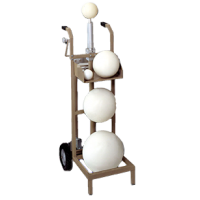
\includegraphics[width=\textwidth]{bss}
\caption{Bonner Sphere Spectrometer}
\end{figure}
\end{column}
\begin{column}{.5\textwidth}
\begin{itemize}
\item Active detection through $^6$Li($n$, $\alpha$)t
\item Thermally sensitive crystal
\item Increasing HDPe sphere sizes provide different (faster) responses.
\end{itemize}
\end{column}
\end{columns}
\end{frame}

%%%%%%%%%%%%%%%%%%%%% gold foil based spectrometers
\begin{frame}
\frametitle{Foil-based Spectrometers}

\begin{itemize}
\item Passive detection through various reactions, [($n$, $\gamma$), ($n$, $\alpha$), etc.]
\item Secondary $\gamma$-ray actually what is measured
\item Multi-foil experiment can span entire spectrum
\item Gold (thermally sensitive) can be used in conjunction with Bonner Spheres \cite{viererbl2012comparison}
\end{itemize}

\end{frame}

%%%%%%%%%%%%%%%%%%%%% the mathematic formulation/unfolding
\begin{frame}
\frametitle{Problem Formulation}
\begin{equation}
\label{eqn:disc-response}
N_k + \epsilon_k = \sum_i R_{ki} \phi_i, \quad k = 1,\ldots, m .
\end{equation}

$N_k$ Measured response of detector $k$\\
$\epsilon_k$ (Unknown) error of detector $k$ response\\
$R_{ki}$ Response function of detector $k$ at energy $i$\\
$\phi_i$ (Unknown) Flux in energy $i$\\
\vspace{0.05\textheight}

Ill posed - much more energy groups than detectors!\\
Infinite solutions!

\end{frame}


%%%%%%%%%%%%%%%%%%%%% how to solve
\begin{frame}
\frametitle{How to Solve}

How do we arrive at one acceptable solution in a domain of infinite solutions?

\begin{itemize}
\item Default Spectrum - becomes a `tuning' problem
\item Maximum Entropy - neutrons behave like gases
\end{itemize}

\end{frame}

%%%%%%%%%%%%%%%%%%%%% unfolding methods
\begin{frame}
\frametitle{Unfolding Methods}

Doroshenko Directed Divergence
\begin{itemize}
\item Minimize Directed Divergence
\item Iterative
\end{itemize}

Gravel
\begin{itemize}
\item Modified Sand-II
\item Iterative
\item Works by applying correction factors to a weighting function
\end{itemize}

MAXED
\begin{itemize}
\item Maximized Skilling entropy, a function of both the default and solution spectrum
\end{itemize}


\end{frame}


%%% NEBP Modeling Effort (10) ---------------------------------------------------------------------------------------
\section{Simulated Work}

%%%%%%%%%%%%%%%%%%%%% modeling steps/overview
\begin{frame}
\frametitle{Simulated Work}

Simulation of the NEBP flux

\end{frame}


%%%%%%%%%%%%%%%%%%%%% modeling steps/overview
\begin{frame}
\frametitle{Modeling Overview}

\begin{itemize}
\item Added NEBP to existing model
\item Tallied fission rates within core to produce SDEF
\item Applied ADVANTG variance reduction software to speedup tally convergence
\item Tallied flux at NEBP aperture
\end{itemize}

\end{frame}

%%%%%%%%%%%%%%%%%%%%% existing model
\begin{frame}
\frametitle{Existing Model}

\begin{figure}
\centering
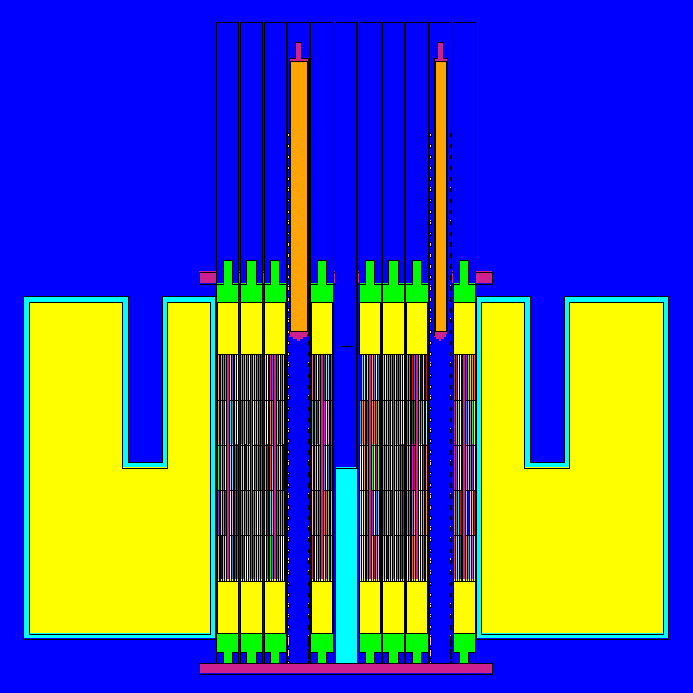
\includegraphics[width = .5\textwidth]{existingyz}
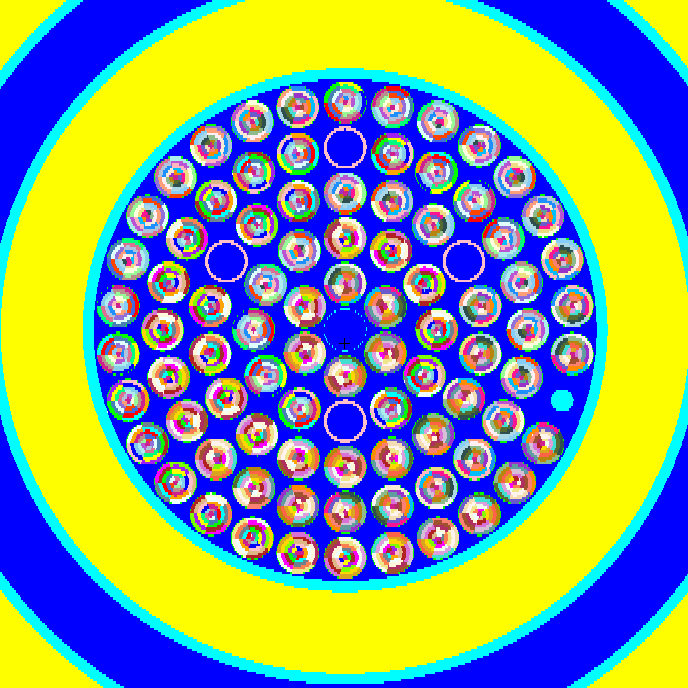
\includegraphics[width = .5\textwidth]{existingxy}
\caption{YZ (left) and XY (right) views of the existing core model with discretized fuel, control rods, graphite reflector, etc.}
\end{figure}

\end{frame}

%%%%%%%%%%%%%%%%%%%%% nebp additions
\begin{frame}
\frametitle{NEBP Additions}

\begin{figure}
\centering
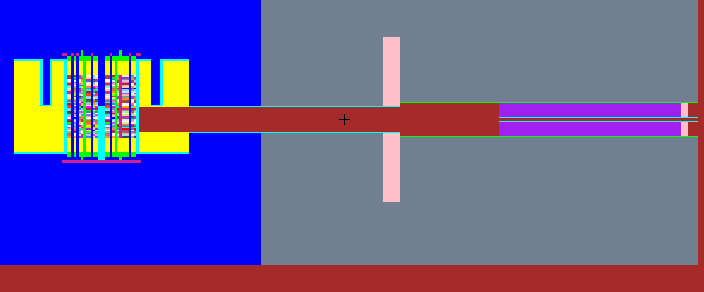
\includegraphics[trim=0 40 0 20, clip, width = .9\textwidth]{mcnp_newxz}\\
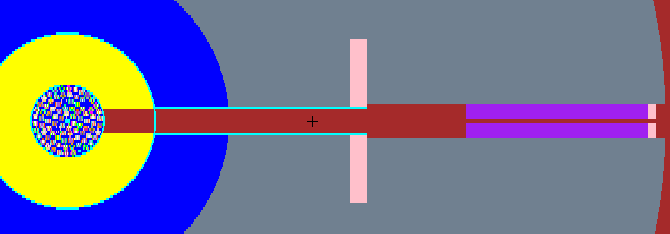
\includegraphics[trim=0 120 0 120, clip, width = .9\textwidth]{mcnp_newxy}
\caption{XZ (top) and XY (bottom) views of the NEBP additions with reflector penetration, lead shadow shield, and collimator.}
\end{figure}

\end{frame}


%%%%%%%%%%%%%%%%%%%%% fission tally
\begin{frame}
\frametitle{Fission Tallys}

\begin{itemize}
\item 40 Axial Segments
\item  5 Radial Segments
\item Used to create PDFs for steady-state problem
\end{itemize}

\end{frame}

%%%%%%%%%%%%%%%%%%%%% fission tally results I
\begin{frame}
\frametitle{Fission Tally Results}

\begin{columns}[c]
\begin{column}{.5\textwidth}
\begin{figure}
\centering
Example results from fission tallies within core fuel, B-ring radial (left), fuel element slice (middle), F-ring axial (right).
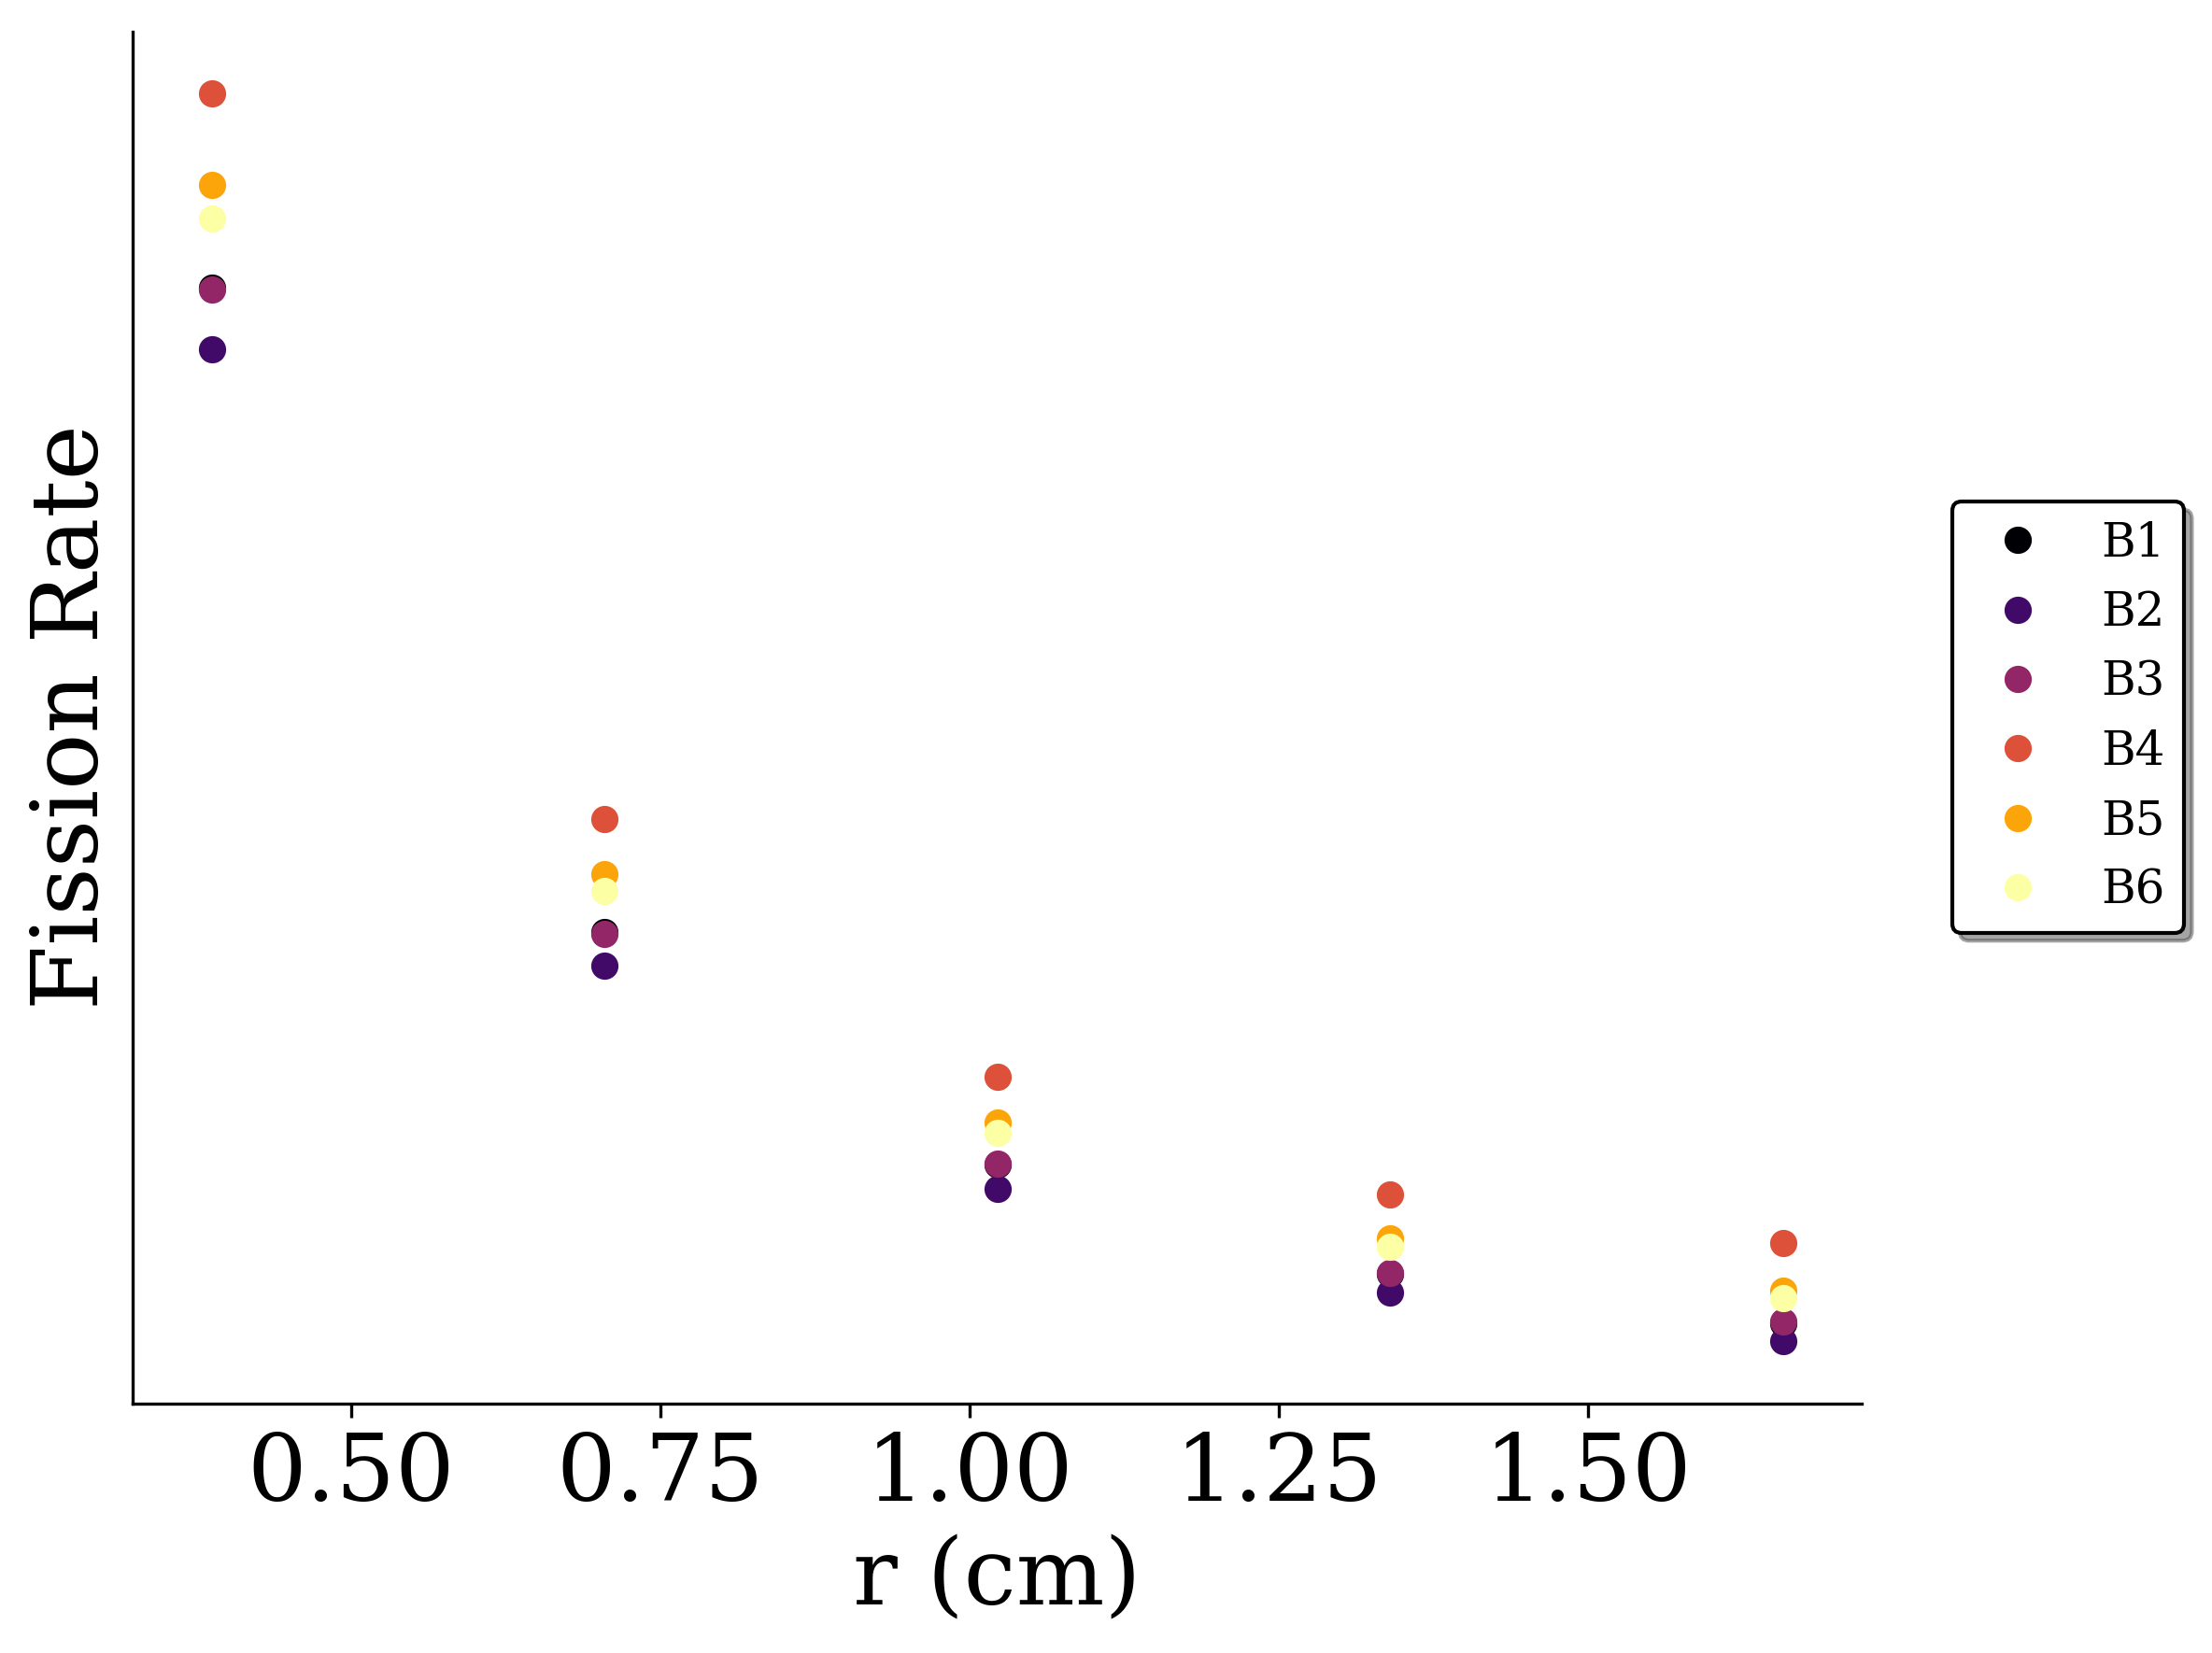
\includegraphics[width = 1.0\textwidth]{radial_rr_density_B}
\end{figure}
\end{column}
\begin{column}{.5\textwidth}
\begin{figure}
\centering
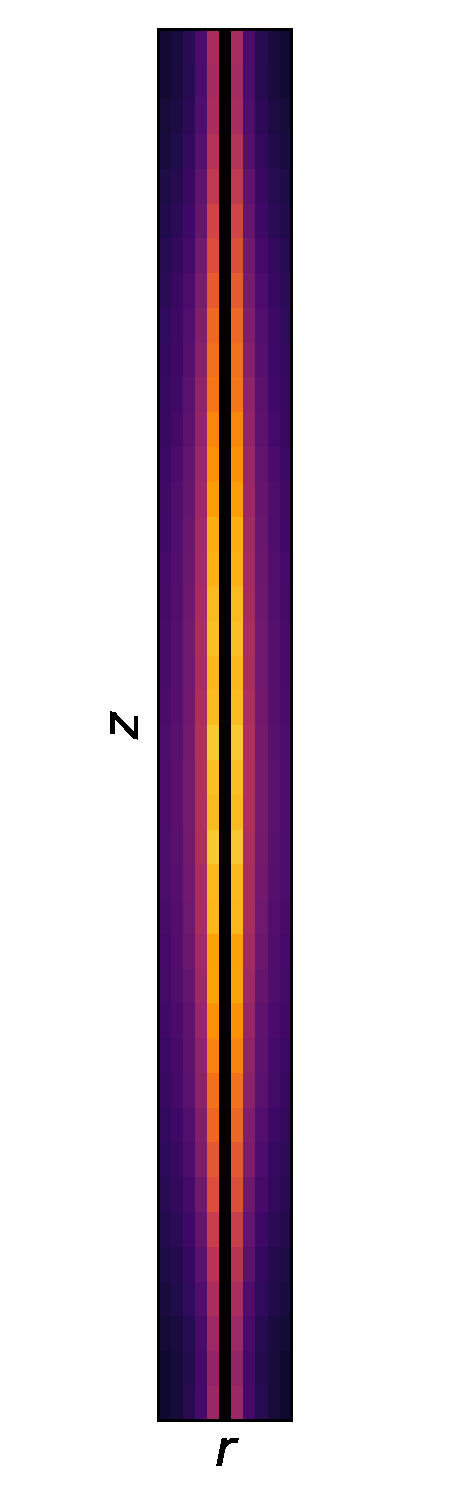
\includegraphics[height = 0.8\textheight]{rr_dist_B1}
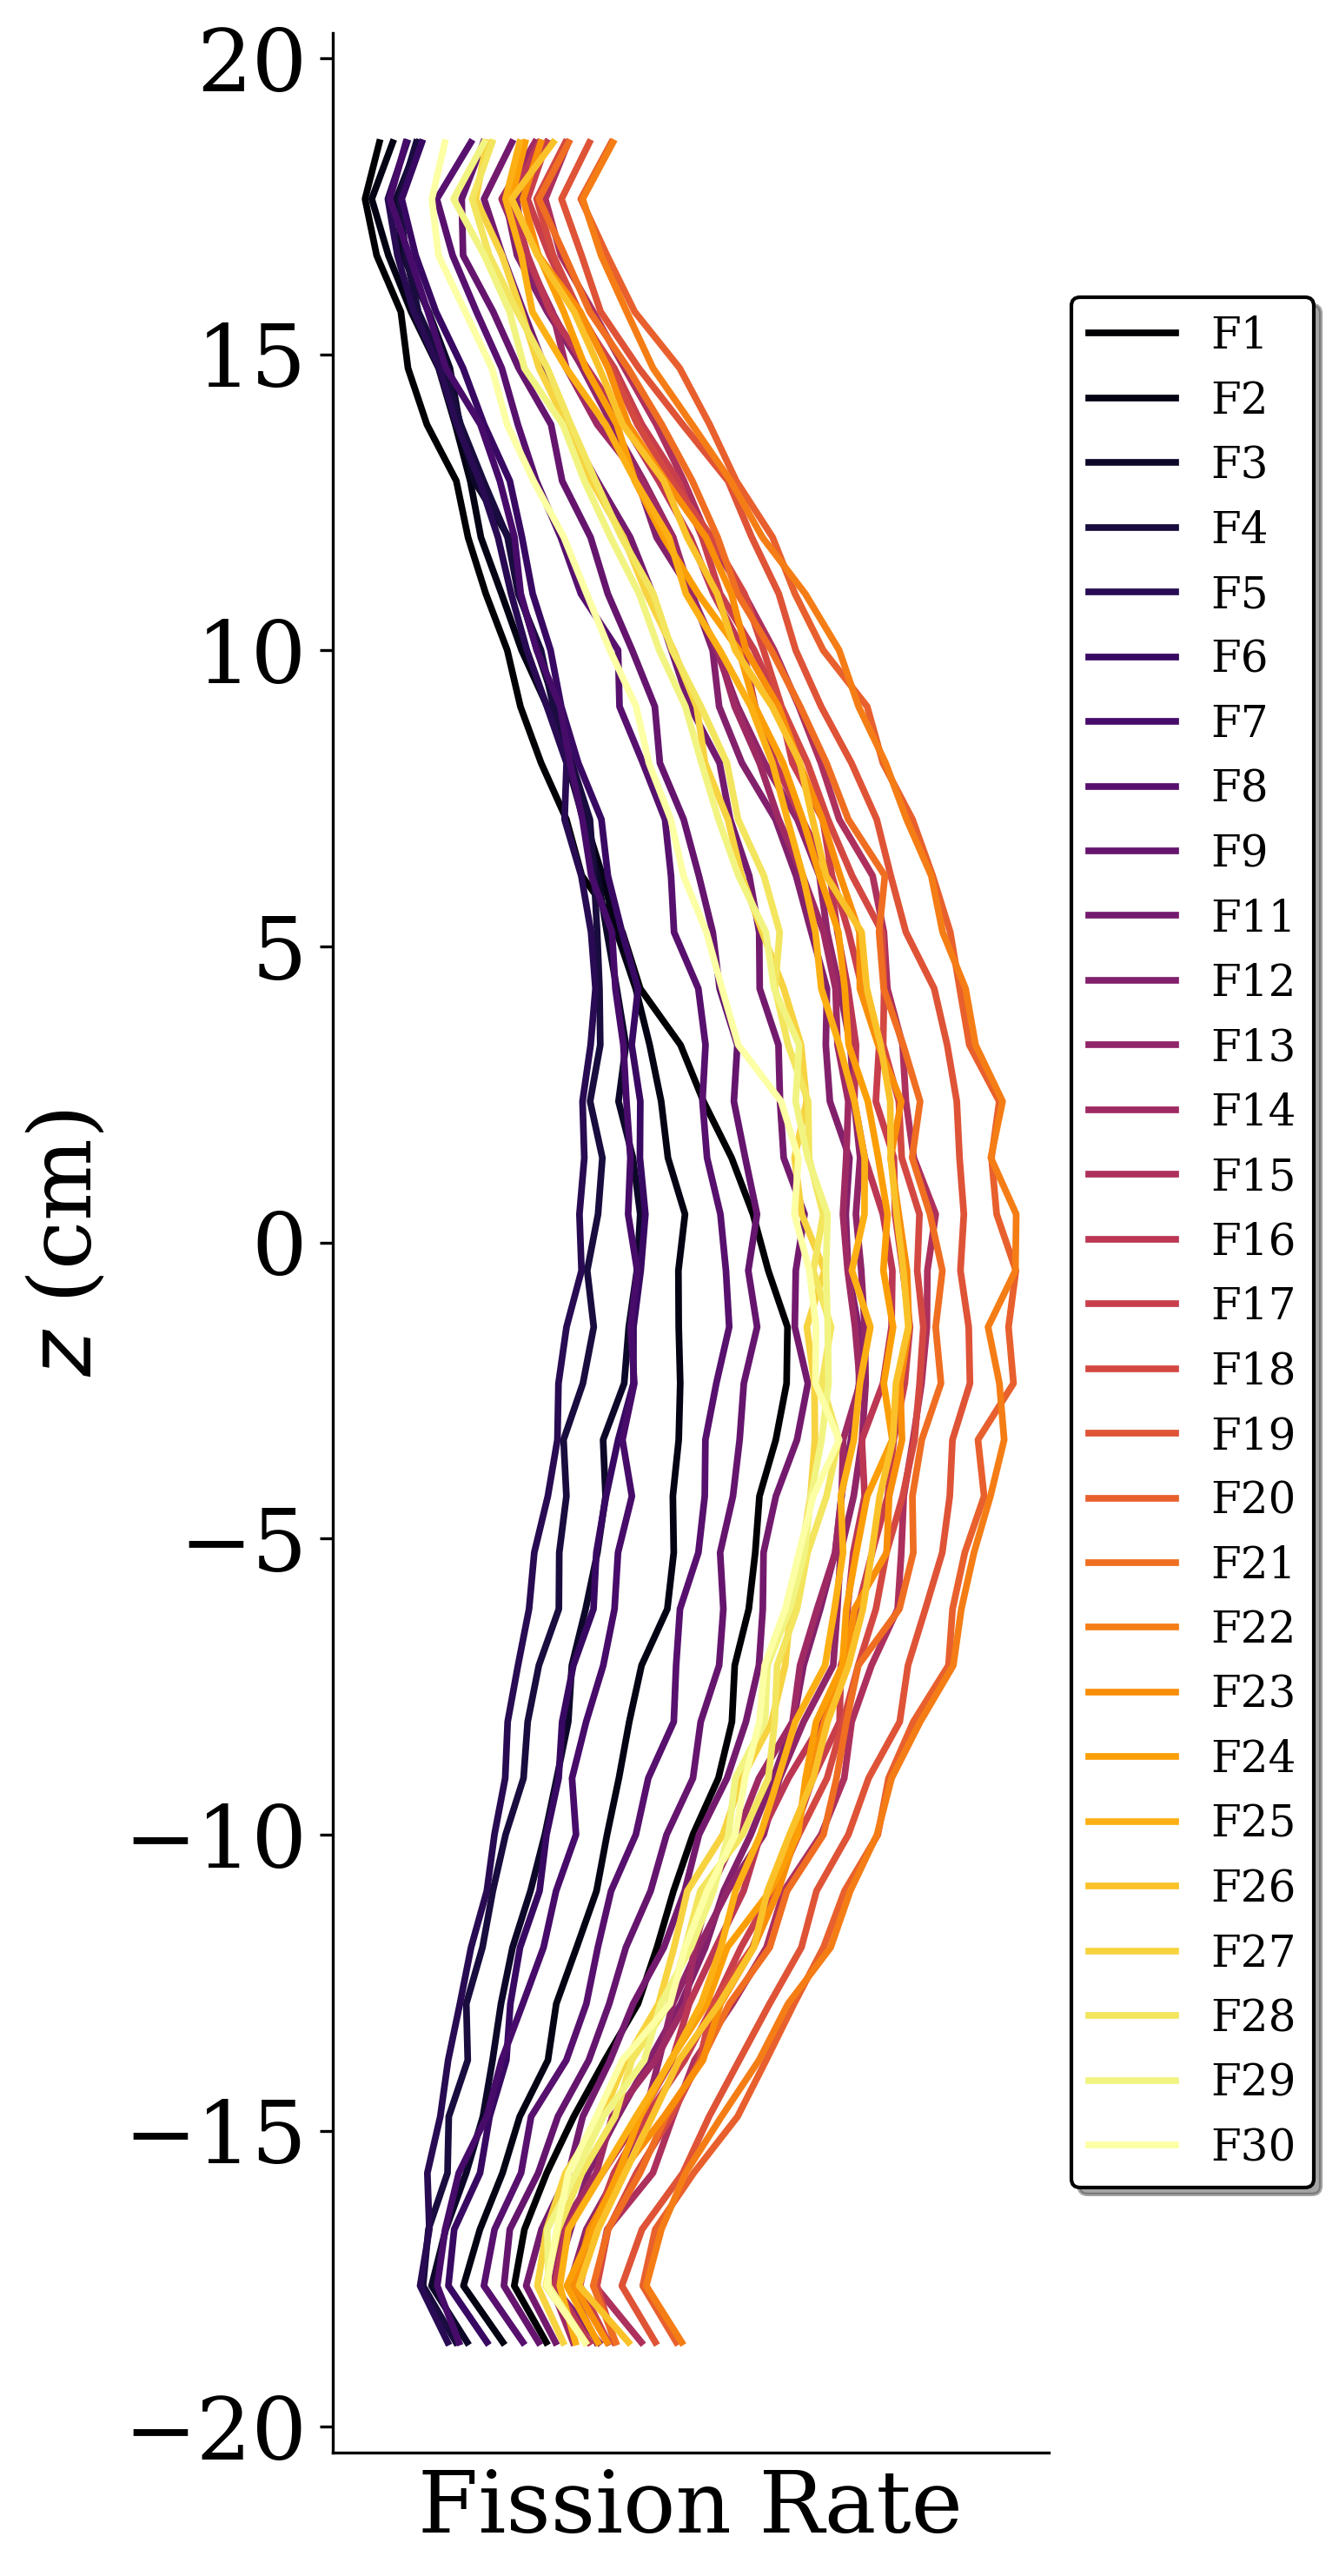
\includegraphics[height = 0.8\textheight]{axial_rr_density_F}
\end{figure}
\end{column}
\end{columns}

\end{frame}

%%%%%%%%%%%%%%%%%%%%% fission tally results II
\begin{frame}
\frametitle{Fission Tally Results}

\begin{figure}
\centering
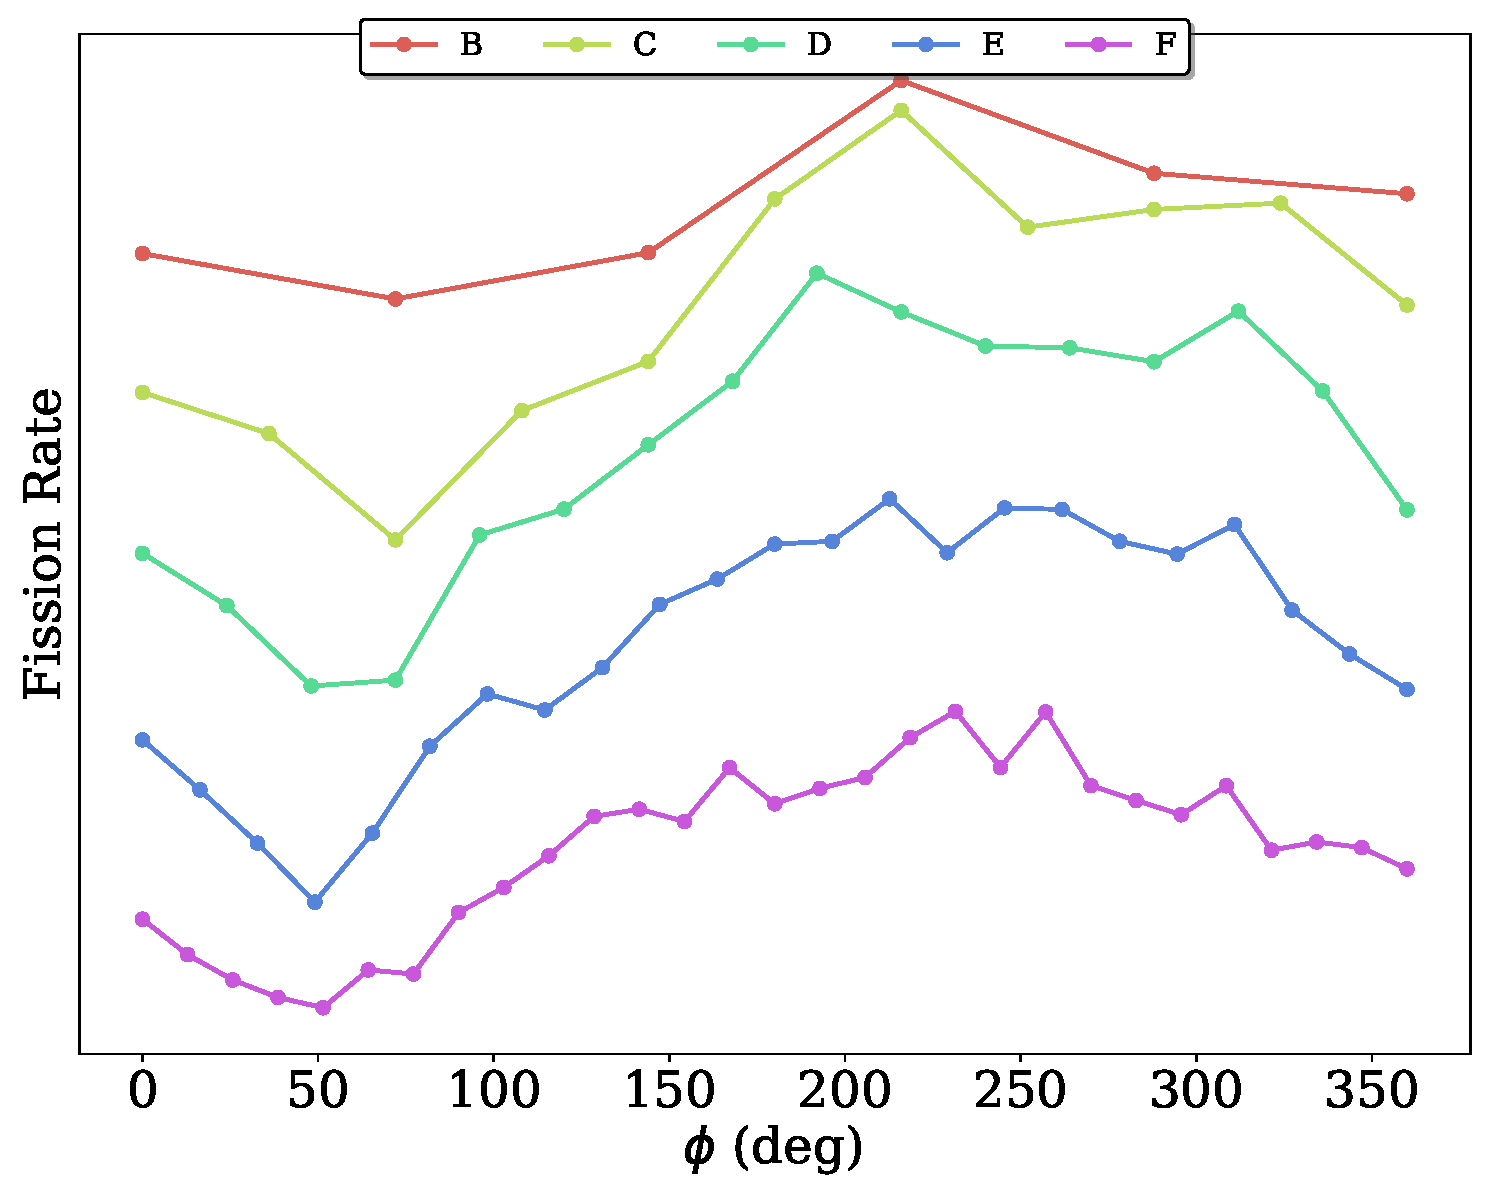
\includegraphics[width = 0.7\textwidth]{totals_azi}
\caption{Integrated fission rates as a function of core azimuthal position.}
\end{figure}

\end{frame}

%%%%%%%%%%%%%%%%%%%%% what is advantg
\begin{frame}
\frametitle{ADVANTG}

The AutomateD VAriaNce reducTion Generator, generates weight window
parameters for a fixed-source, continuous-energy MCNP problem

\begin{itemize}
\item Used Denovo discrete ordinates solver
\item Produces weight windows to speed tally convergence
\item Also adds source biasing parameters to MCNP input
\end{itemize}

\end{frame}

%%%%%%%%%%%%%%%%%%%%% applyting advantg
\begin{frame}
\frametitle{Applying ADVANTG}

\begin{itemize}
\item Model rotated so beam was on $x$-axis
\item 1,570,624 voxels
\item Parallelized for 64 cores
\end{itemize}

\end{frame}

%%%%%%%%%%%%%%%%%%%%% energy distribution
\begin{frame}
\frametitle{Spectral Flux}

\begin{figure}
\centering
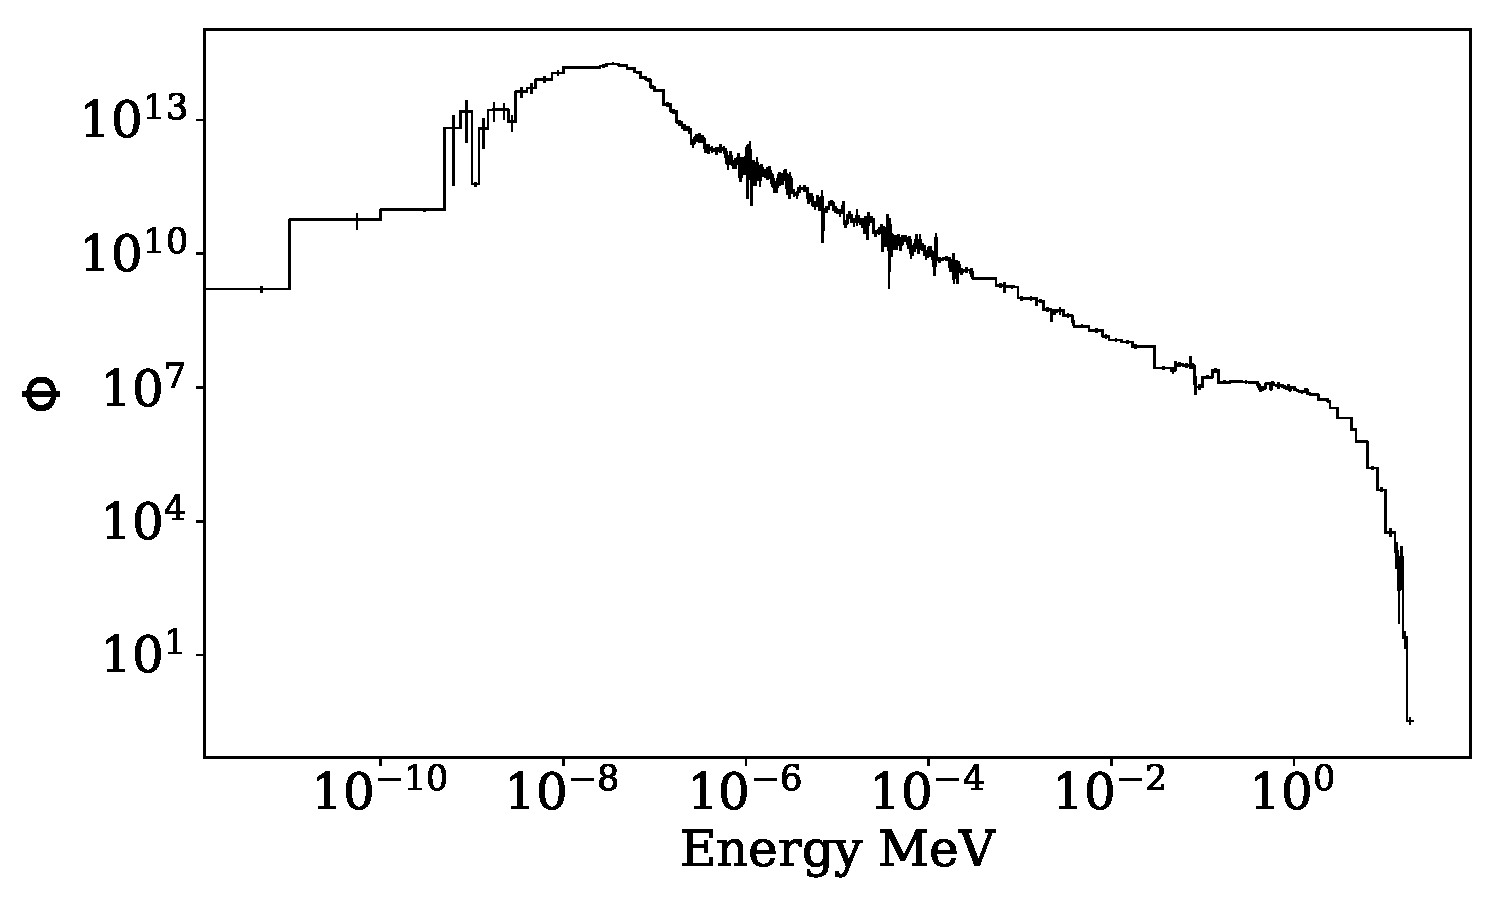
\includegraphics[width = 0.5\textwidth]{flux_erg}
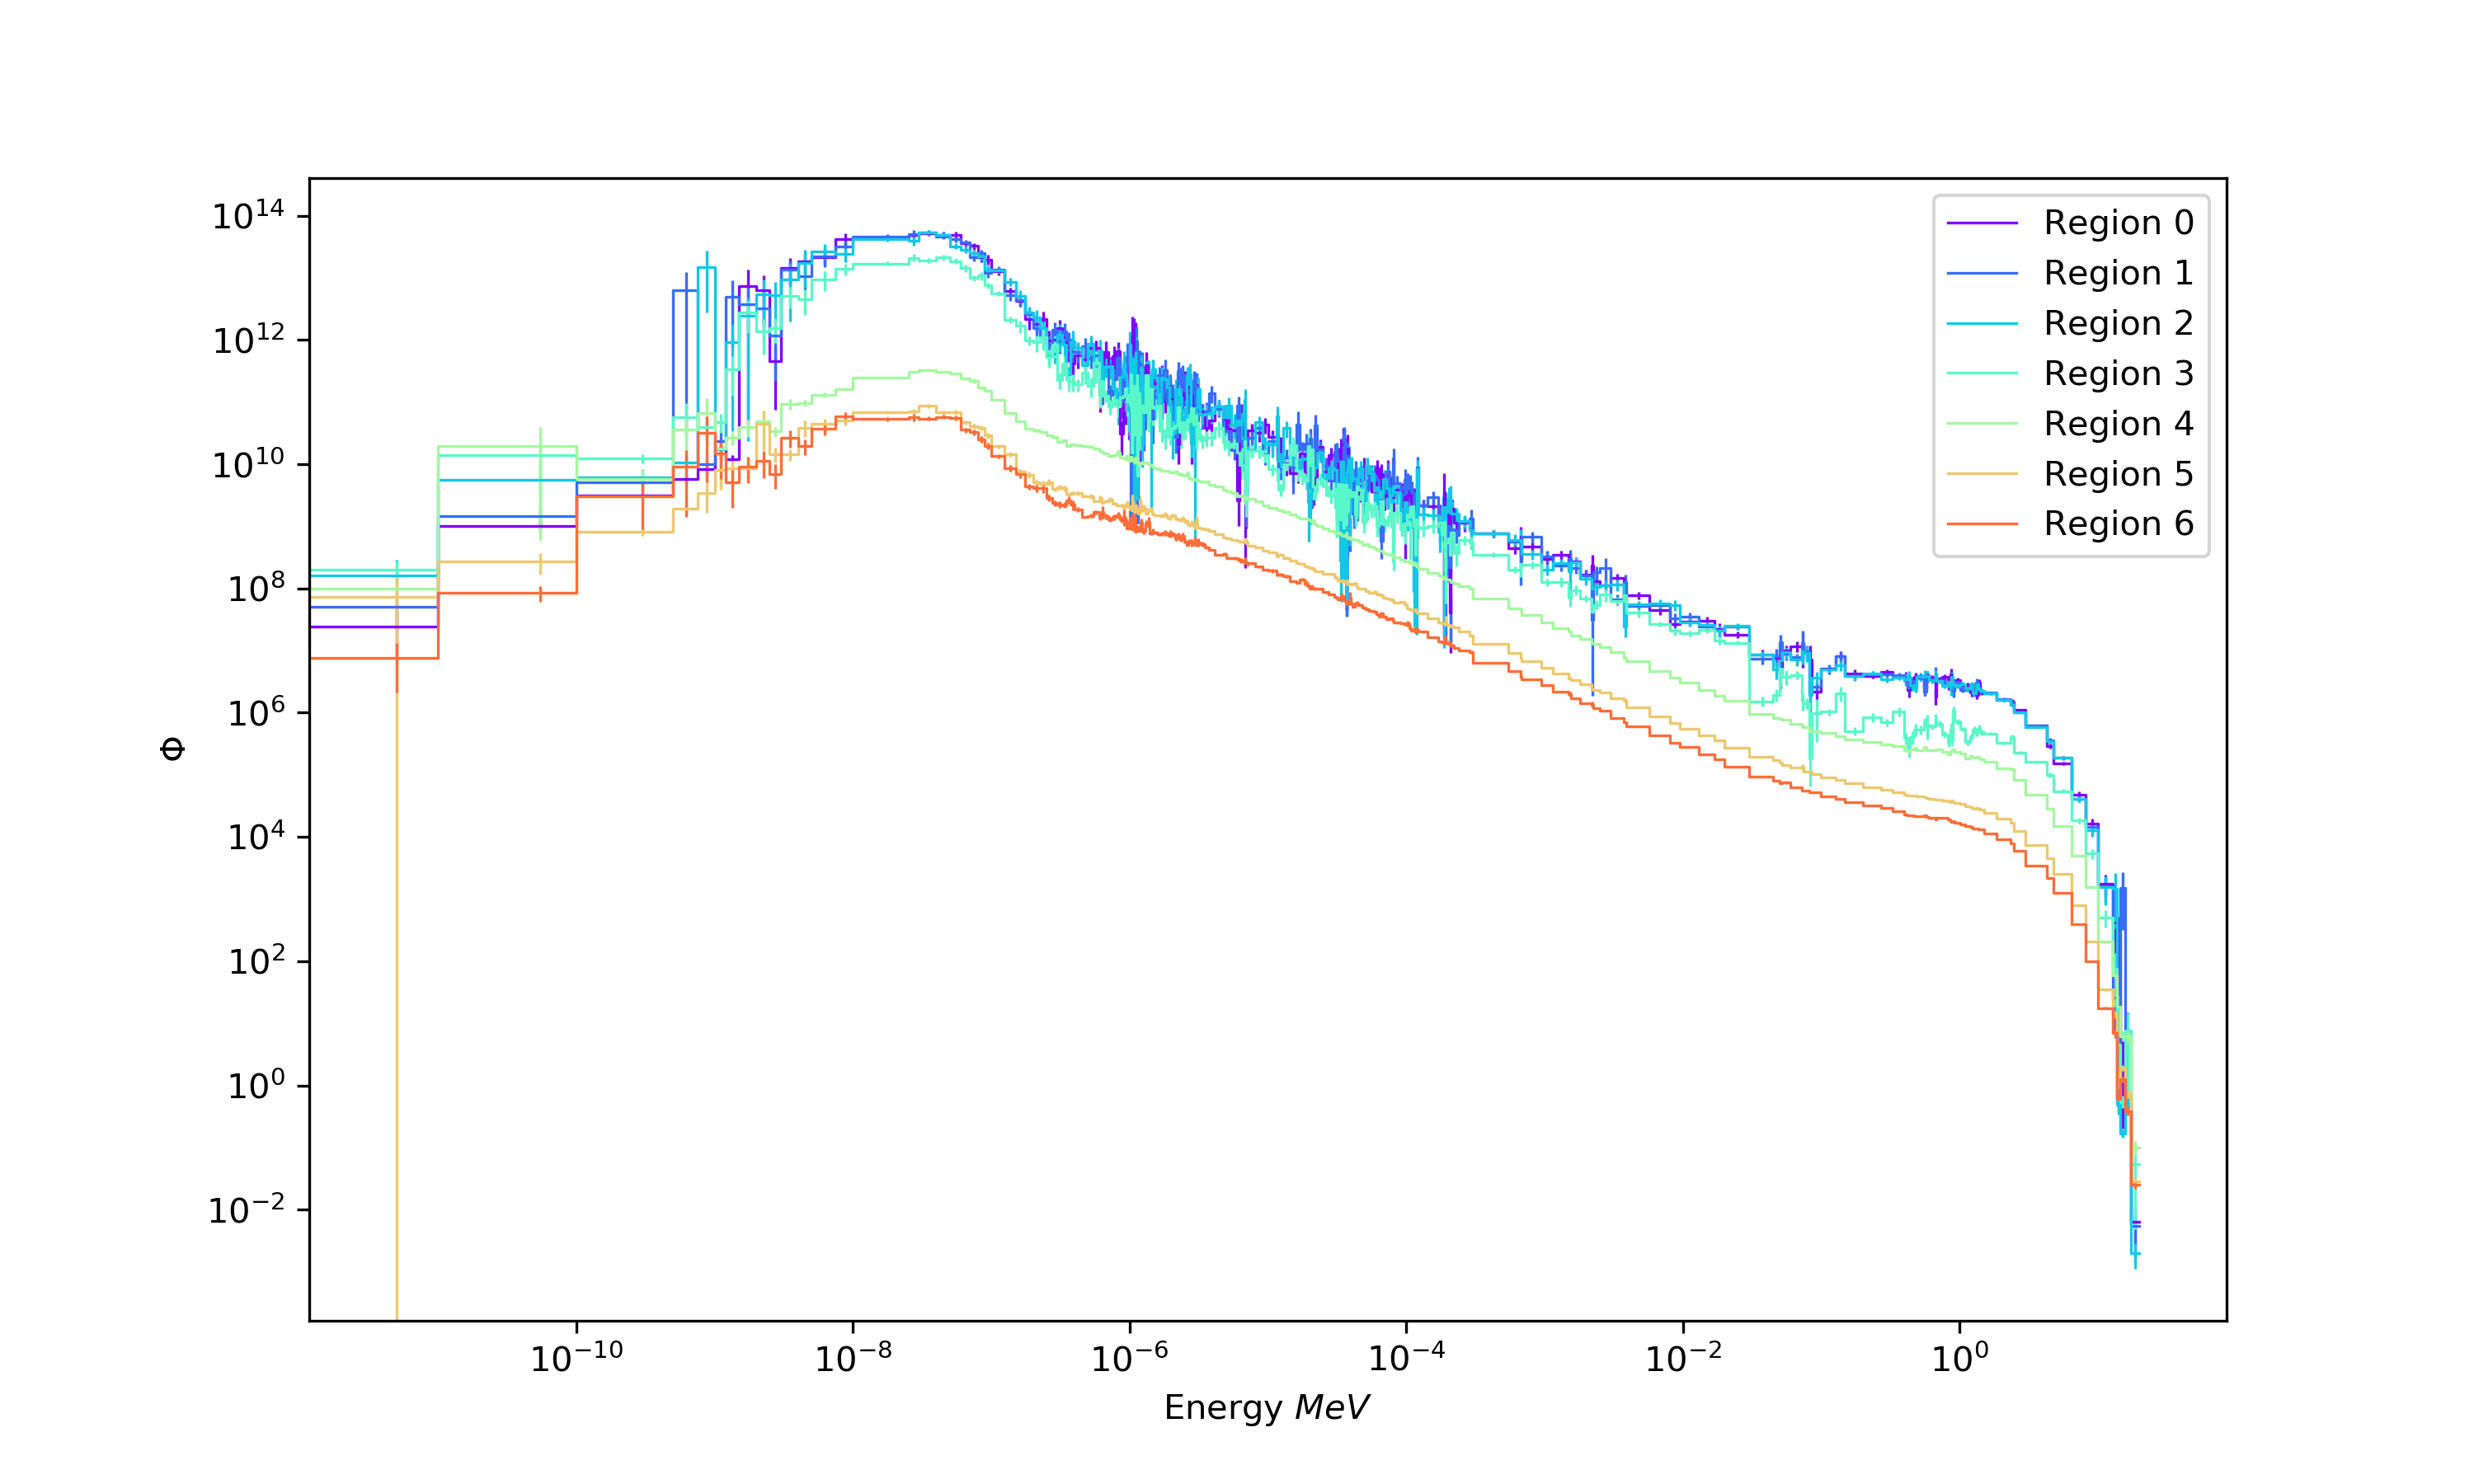
\includegraphics[width = 0.5\textwidth]{flux_rad_erg}
\caption{The spectral flux distribution integrated (left) and separated by radial region (right)}
\end{figure}

\end{frame}

%%%%%%%%%%%%%%%%%%%%% cosine distribution
\begin{frame}
\frametitle{Angular Flux}

\begin{figure}
\centering
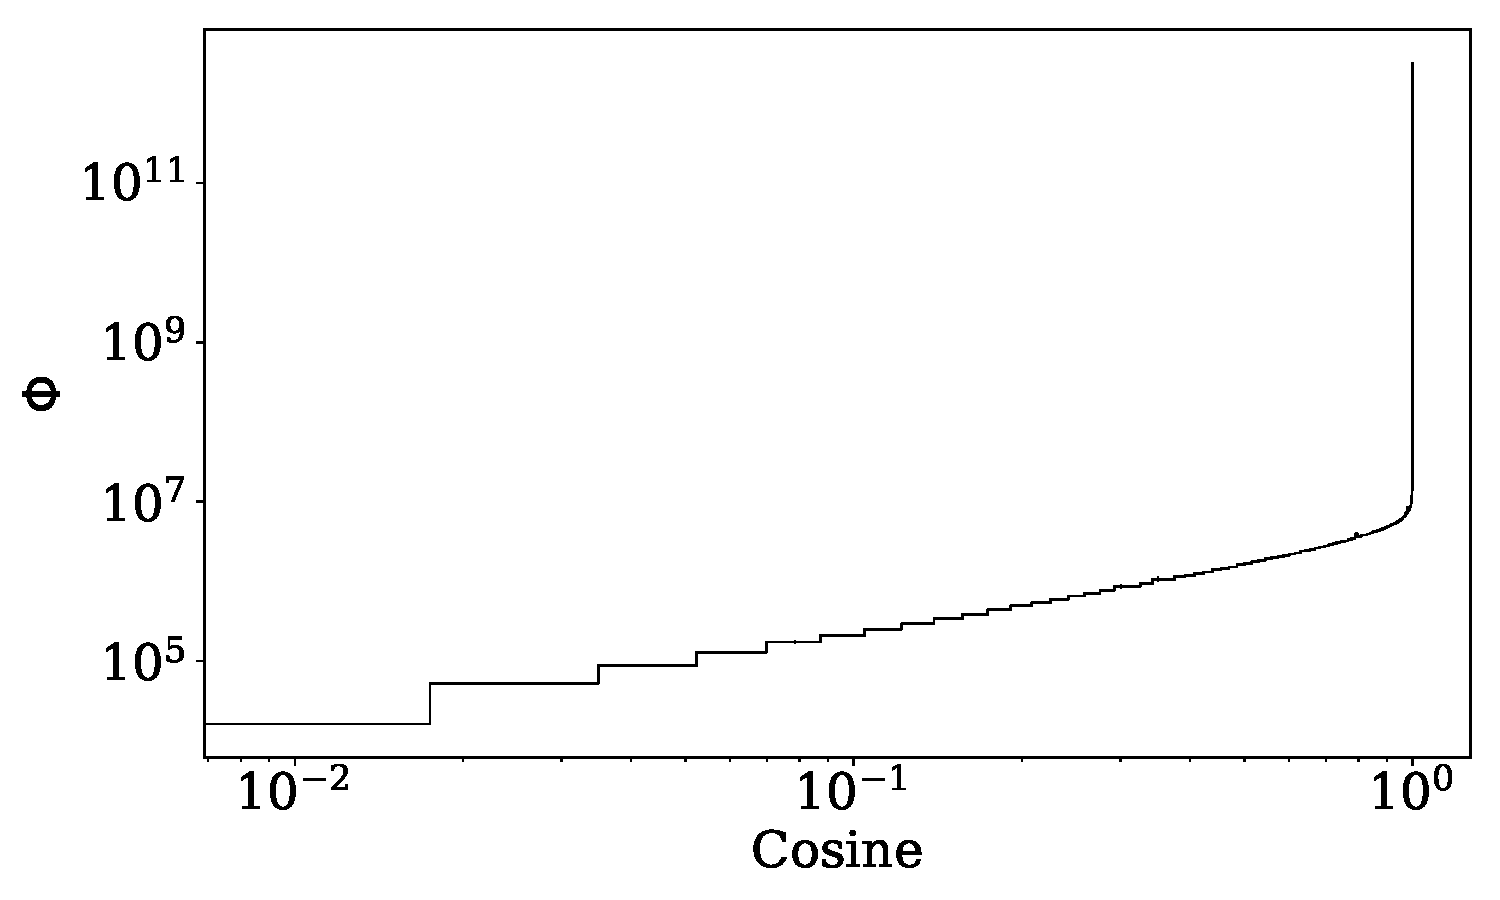
\includegraphics[width = 0.5\textwidth]{flux_cos}
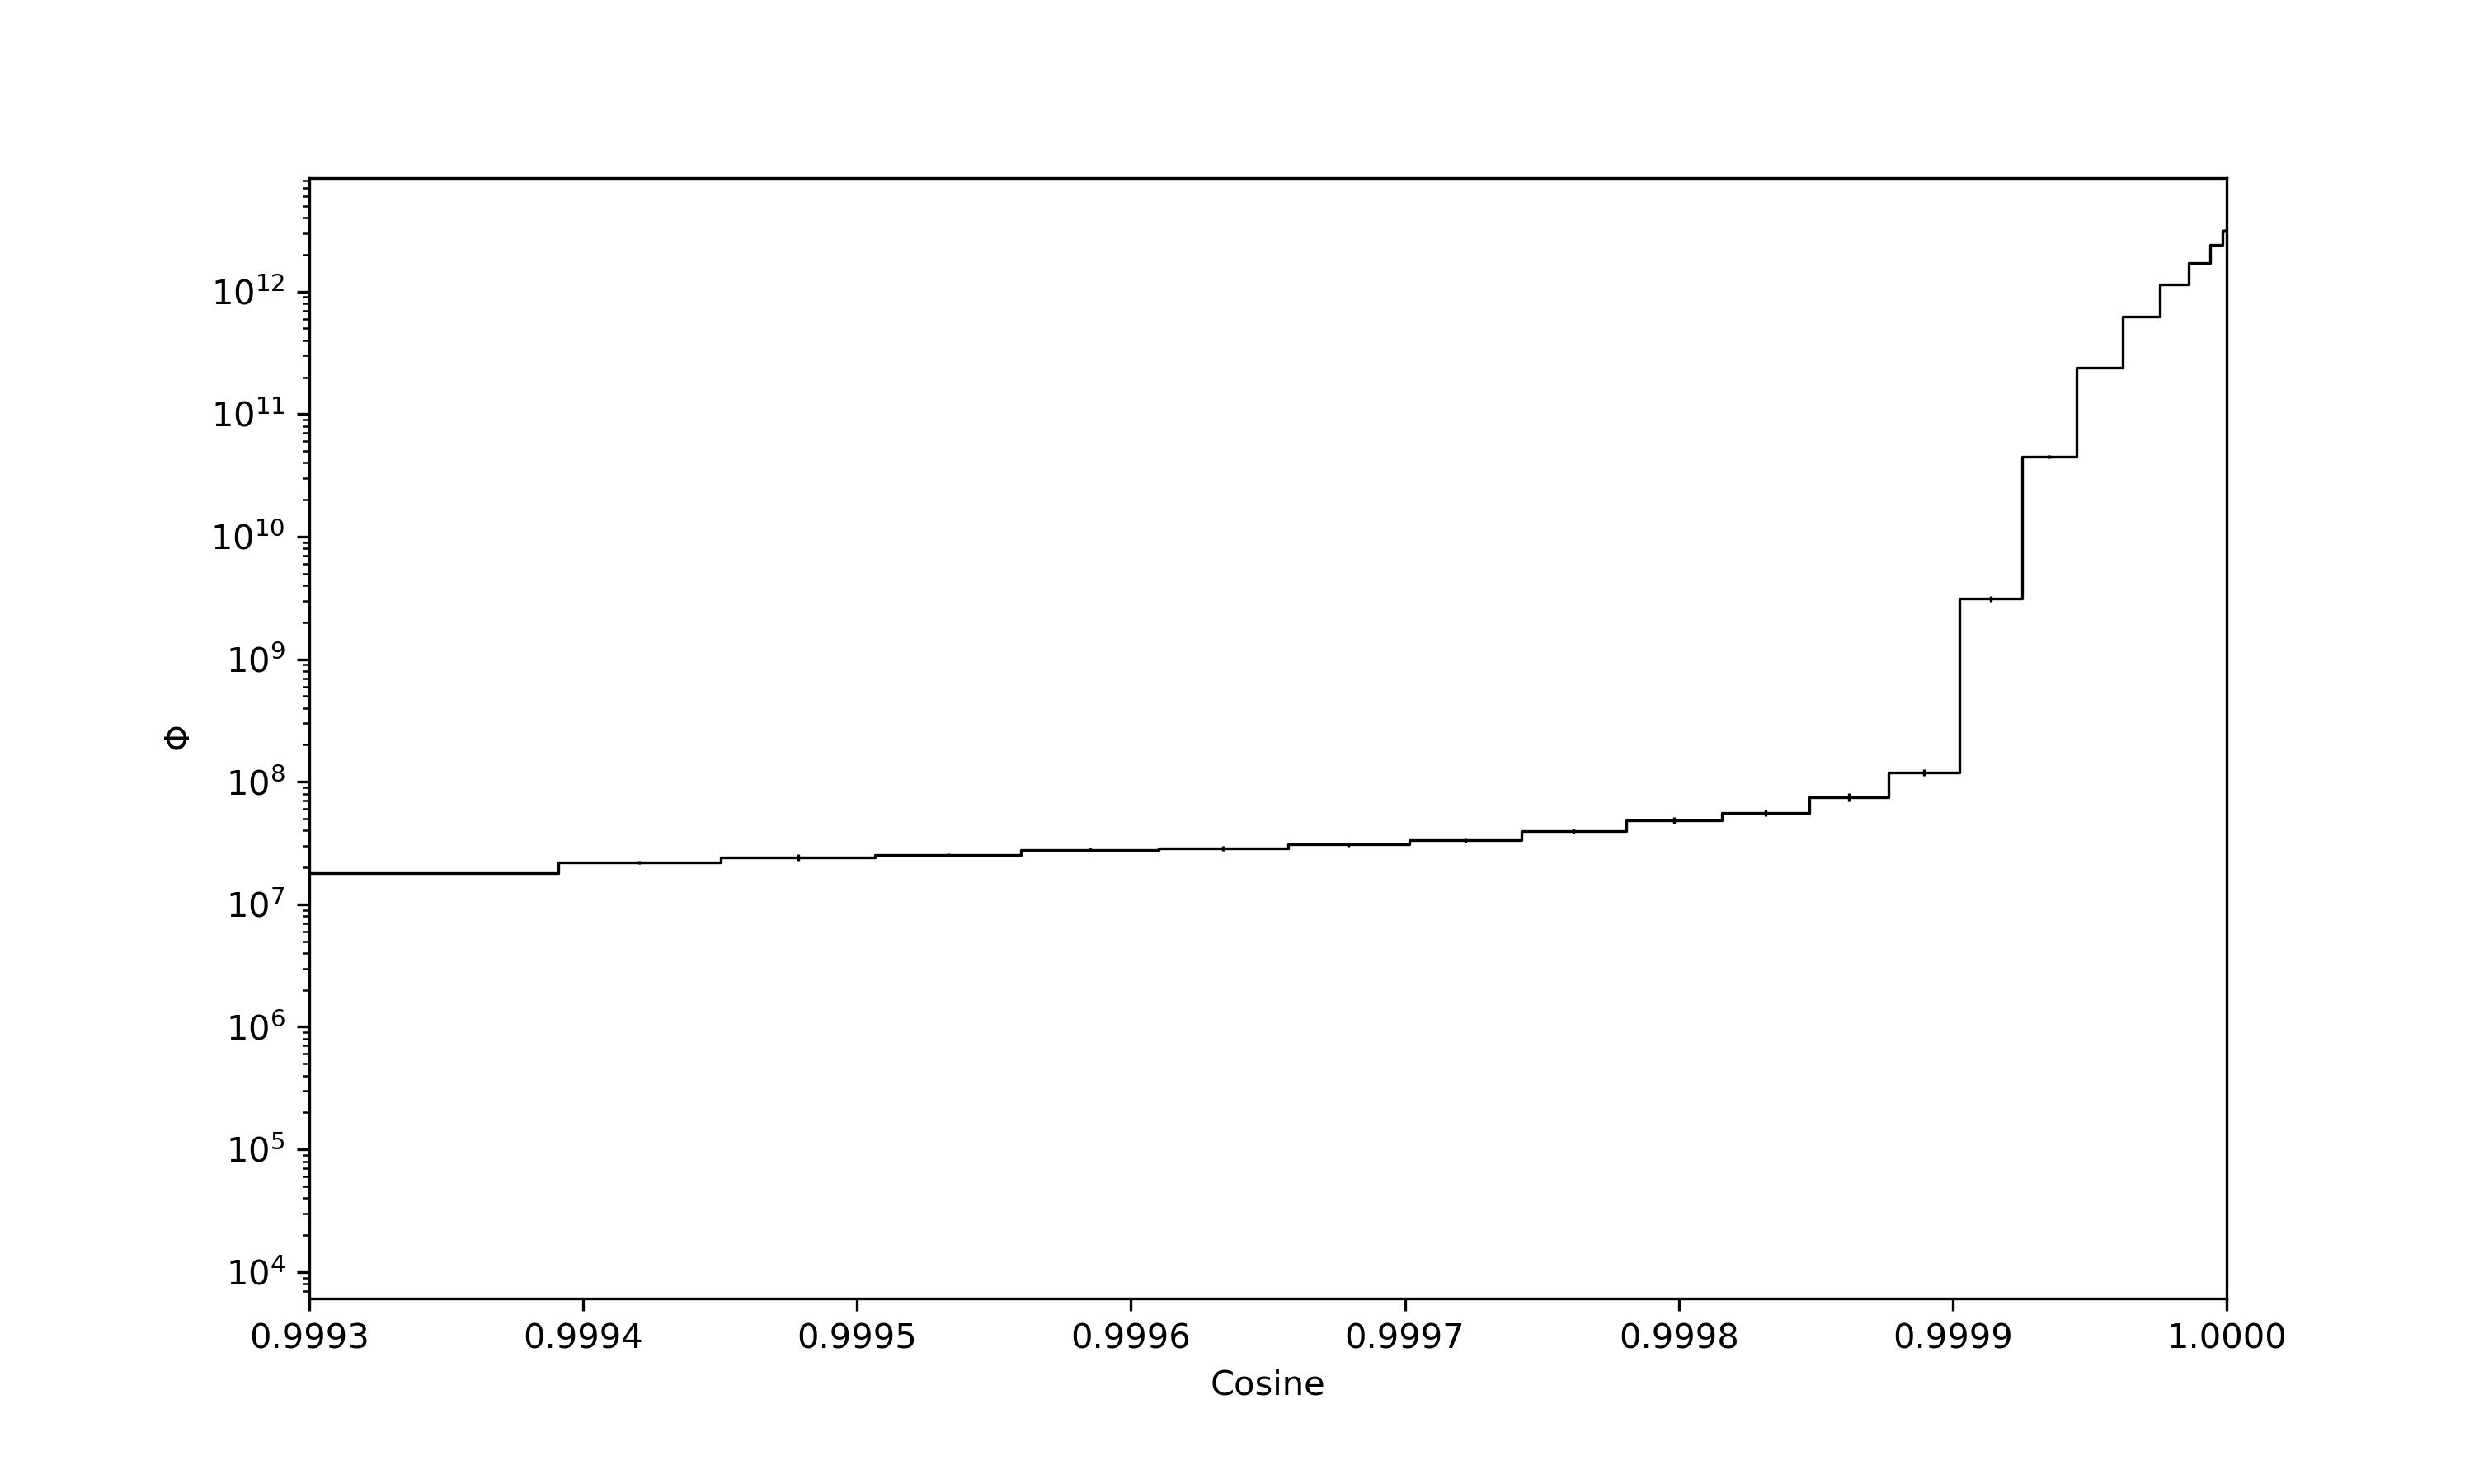
\includegraphics[width = 0.5\textwidth]{flux_cos_detail}
\caption{The angular flux (left) and a zoomed-in view of the angular flux (right).}
\end{figure}

\end{frame}

\begin{frame}
\frametitle{Angular Flux}

\begin{figure}
\centering
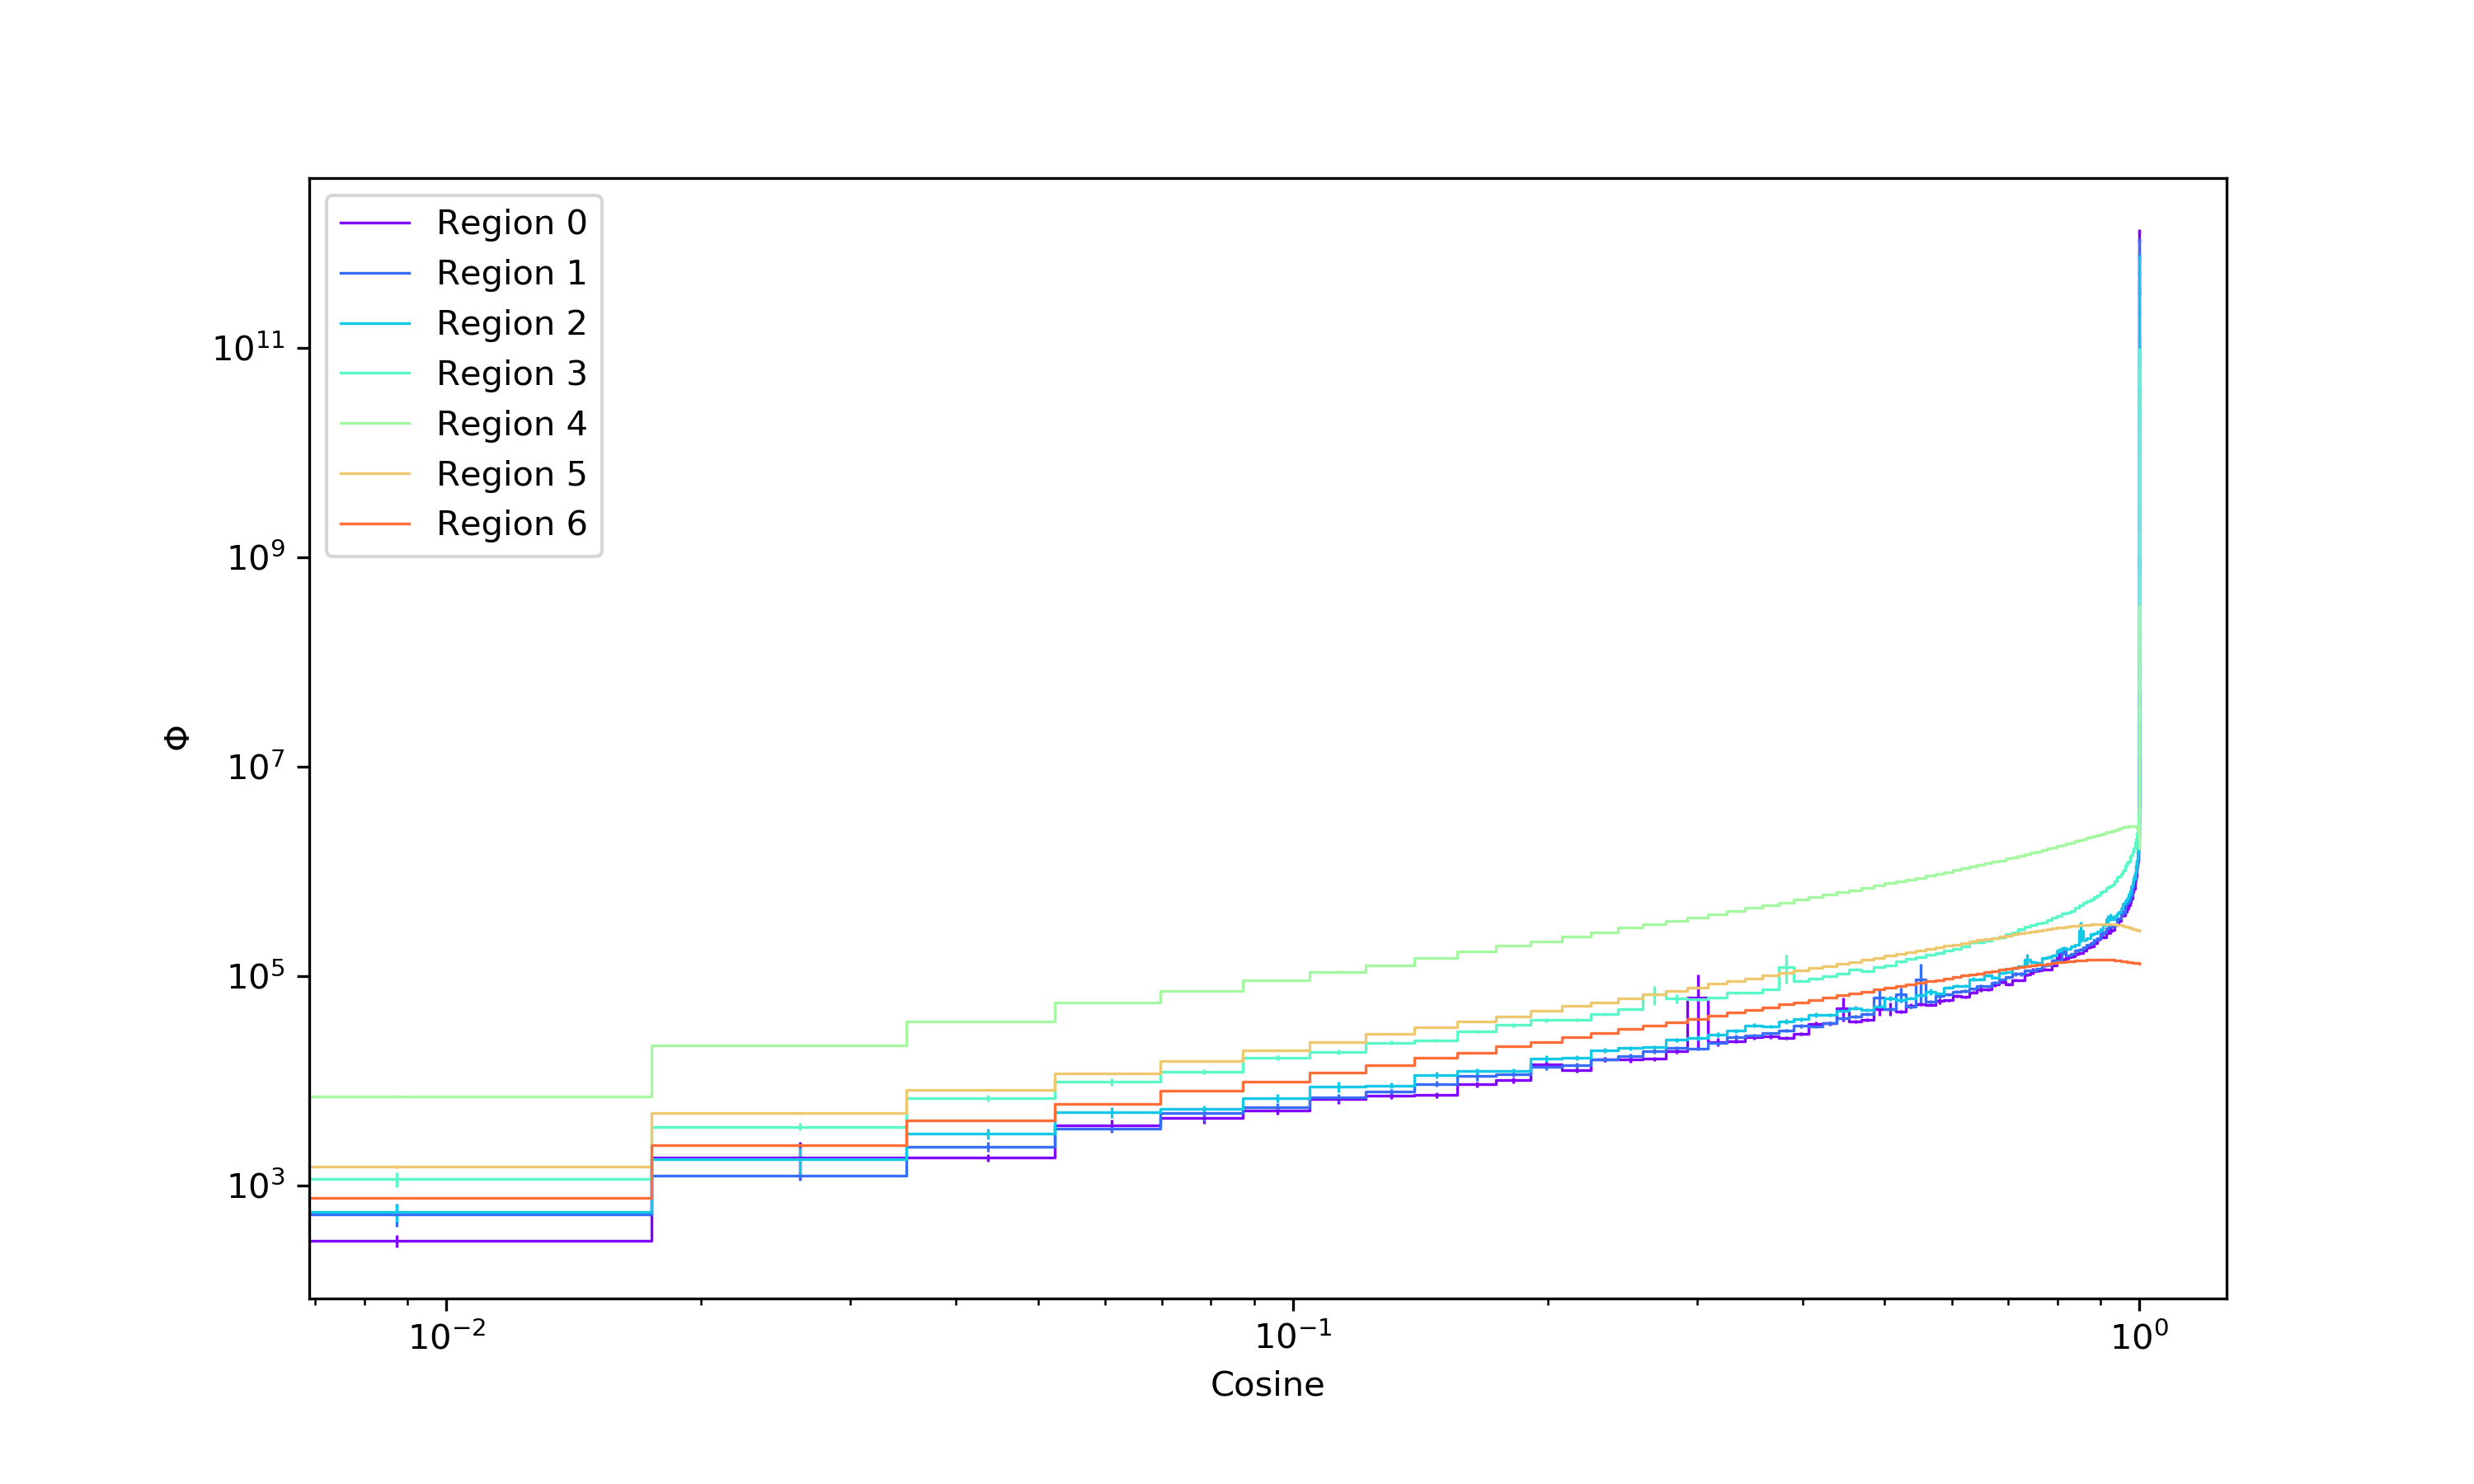
\includegraphics[width = 0.5\textwidth]{flux_rad_cos}
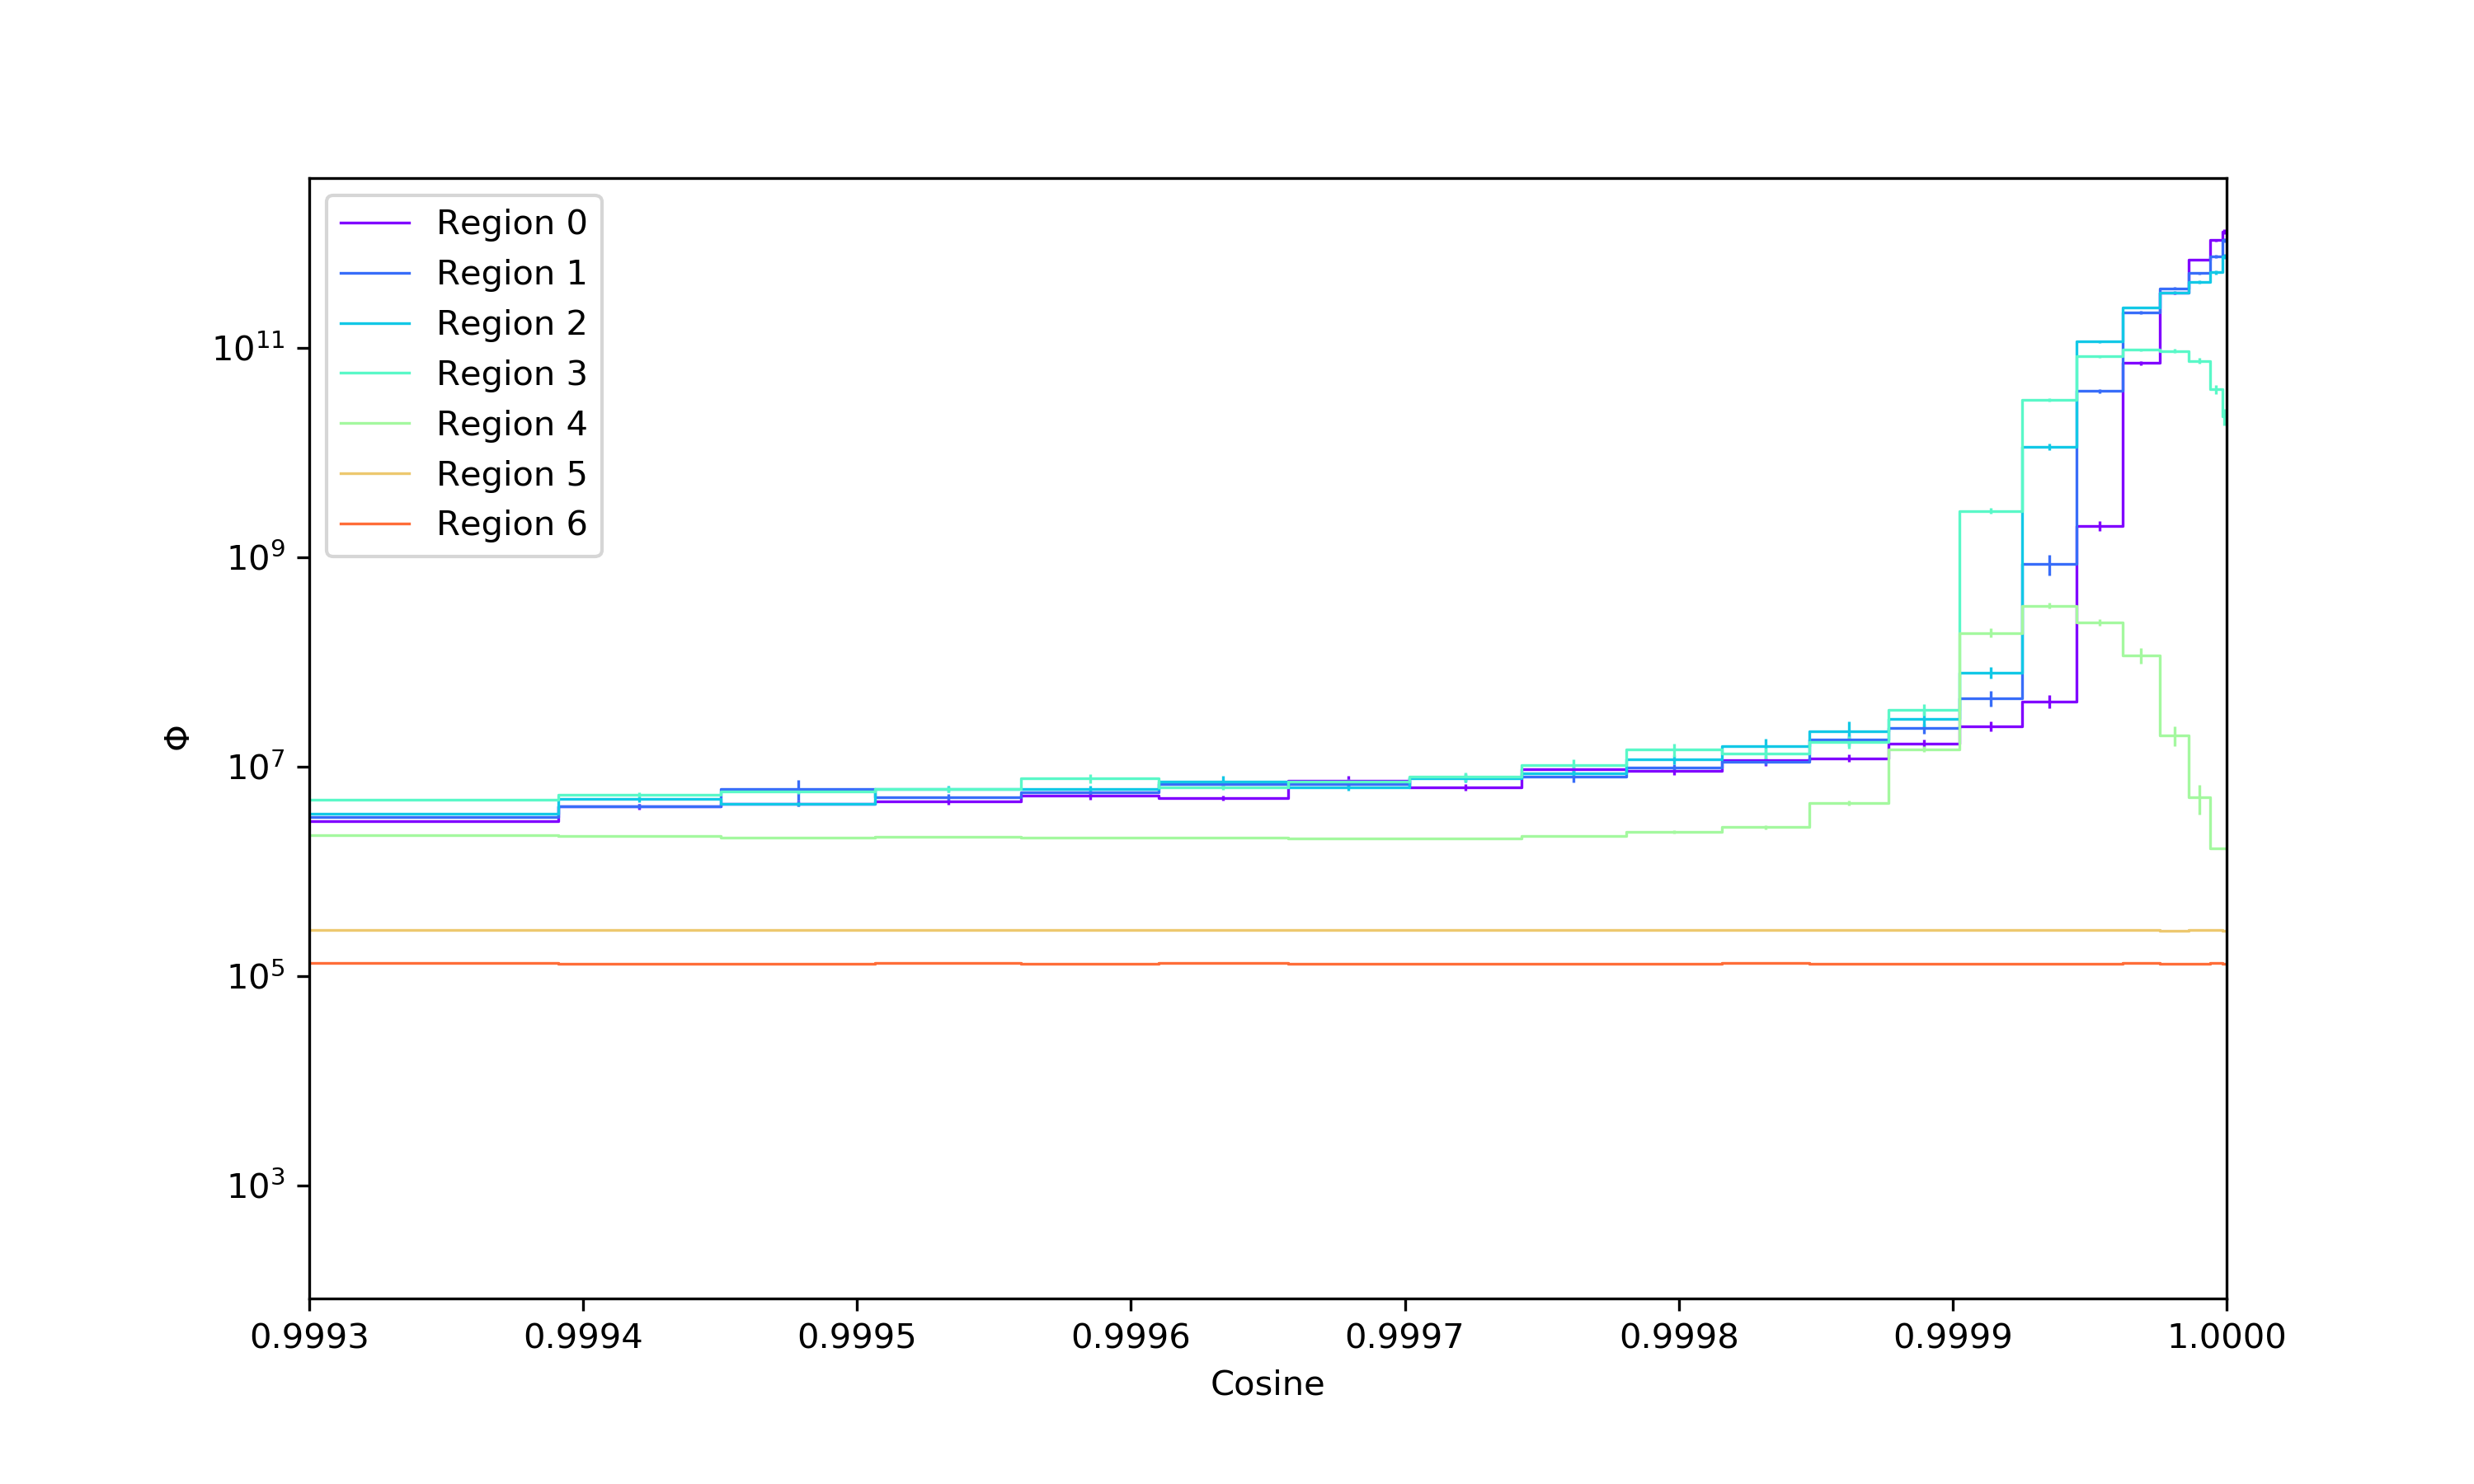
\includegraphics[width = 0.5\textwidth]{flux_rad_cos_detail}
\caption{The angular flux, broken into radial regions (left) and a detail view of the same spectra (right).}
\end{figure}

\end{frame}

%%%%%%%%%%%%%%%%%%%%% radial distribution
\begin{frame}
\frametitle{Radial Flux}

\begin{figure}
\centering
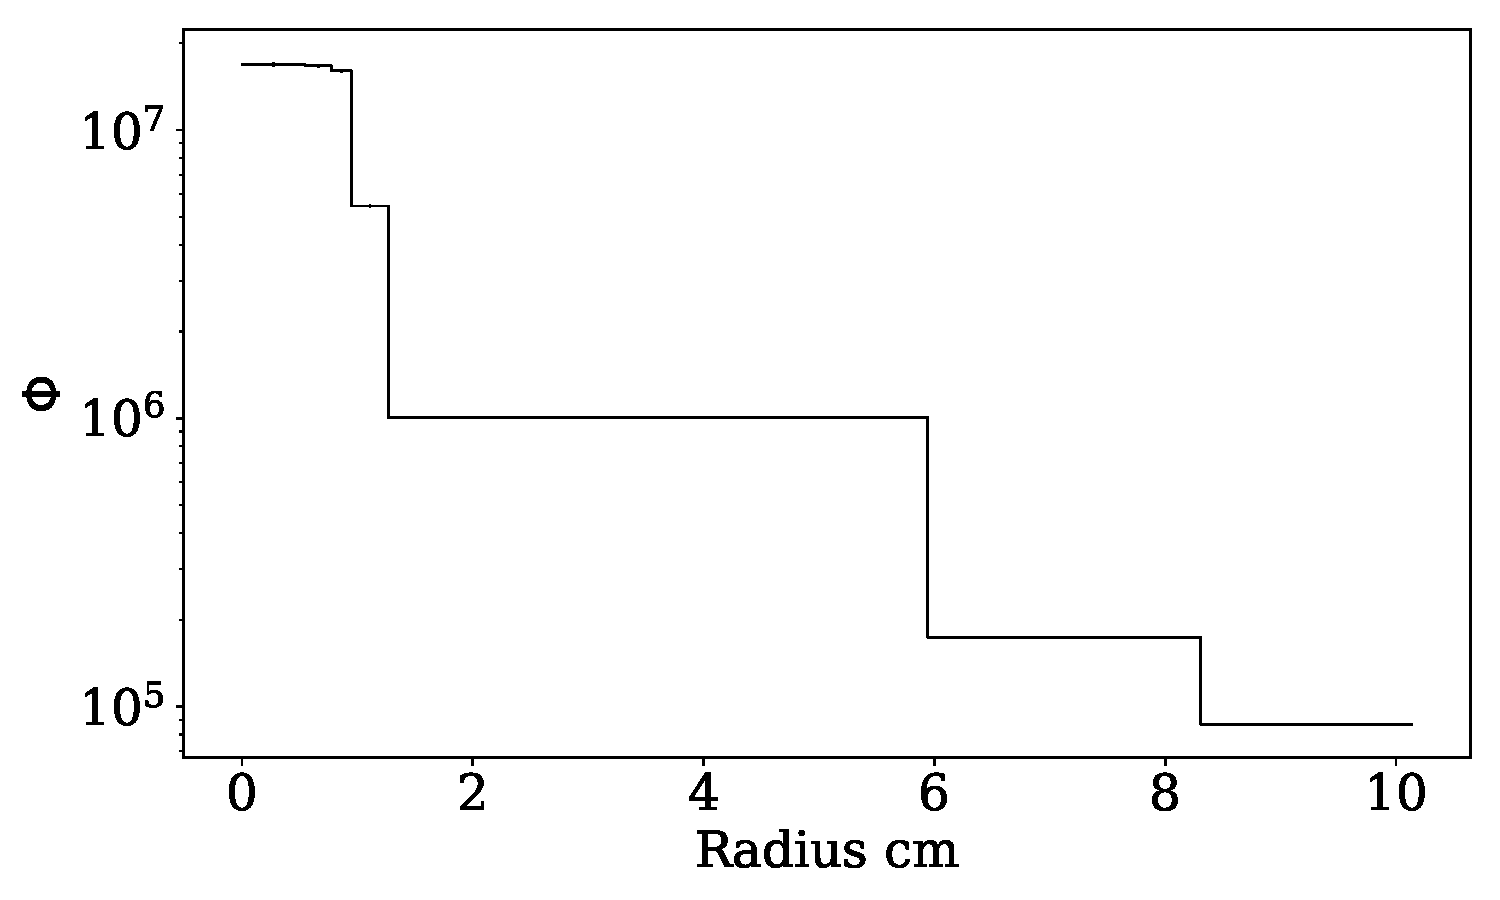
\includegraphics[width = 0.8\textwidth]{flux_rad}
\caption{The energy- and angle-integraded radial flux.}
\end{figure}

\end{frame}

%%% NEBP Experimental Campaign (14) ---------------------------------------------------------------------------------------
\section{Experimental Work}
%%%%%%%%%%%%%%%%%%%%% experimental work
\begin{frame}
\frametitle{Experimental Work}

The effort to experimentally determine the spectral flux of the NEBP.


\end{frame}

%%%%%%%%%%%%%%%%%%%%% modeling steps
\begin{frame}
\frametitle{Gold Foil Tube}

\begin{figure}
\centering
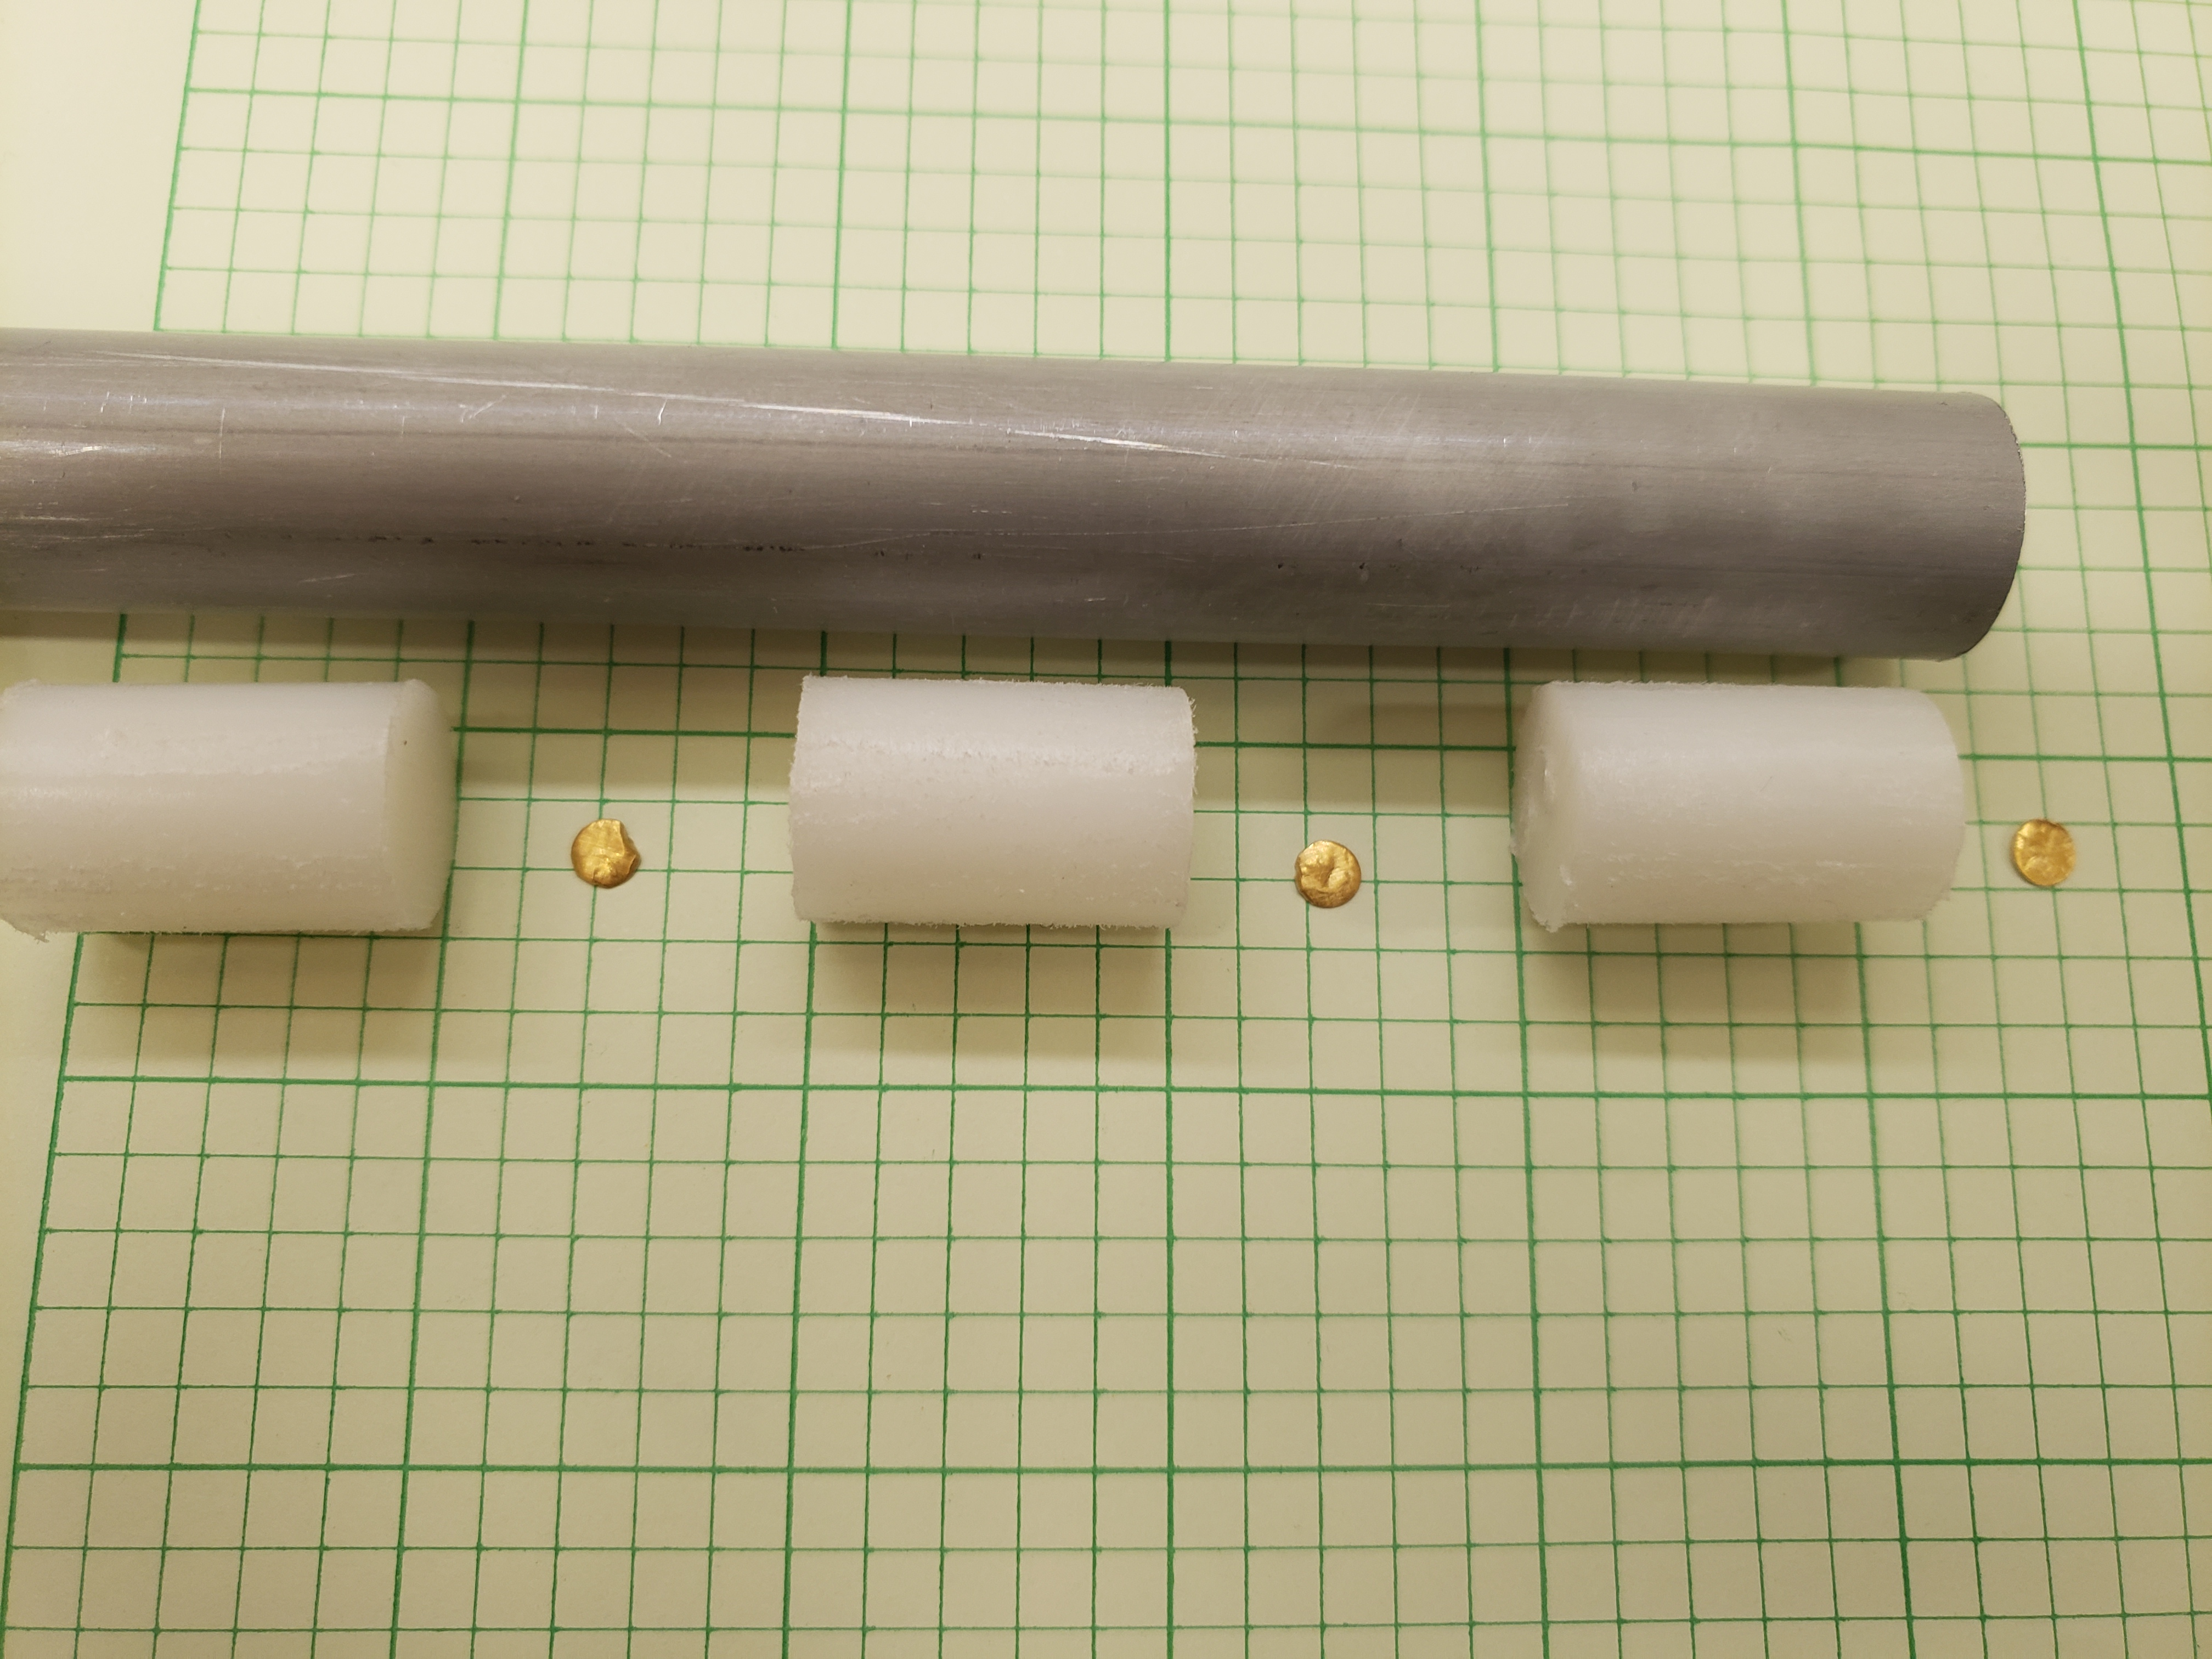
\includegraphics[width = 0.8\textwidth]{foil_tube}
\caption{The disassembled gold foil tube}
\end{figure}


\end{frame}

%%%%%%%%%%%%%%%%%%%%% modeling steps
\begin{frame}
\frametitle{Response Function Generation}

\begin{figure}
\centering
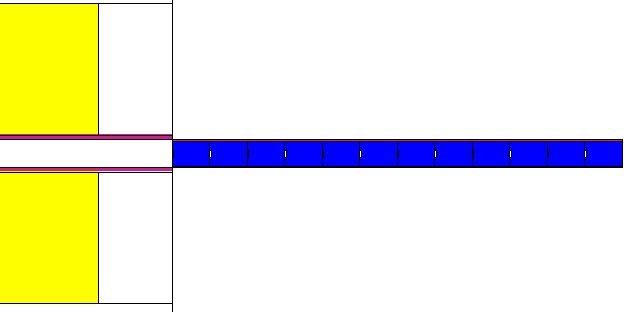
\includegraphics[width = 0.5\textwidth]{mcnpft}
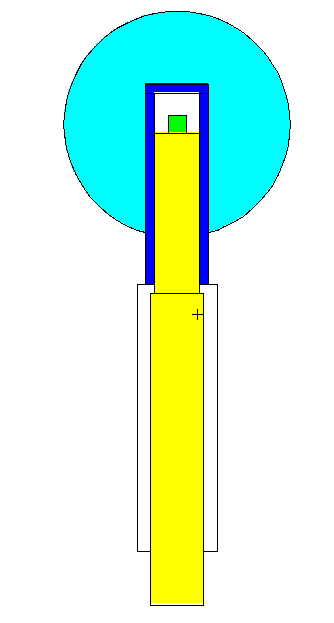
\includegraphics[height = 0.4\textheight]{bonner}
\caption{The foil tube model (left) and the bonner sphere model (right).}
\end{figure}


\begin{itemize}
\item Decoupled MCNP model used to generate response functions
\end{itemize}



\end{frame}

%%%%%%%%%%%%%%%%%%%%% foil tube response functions
\begin{frame}
\frametitle{Foil Tube Response Functions}

\begin{figure}
\centering
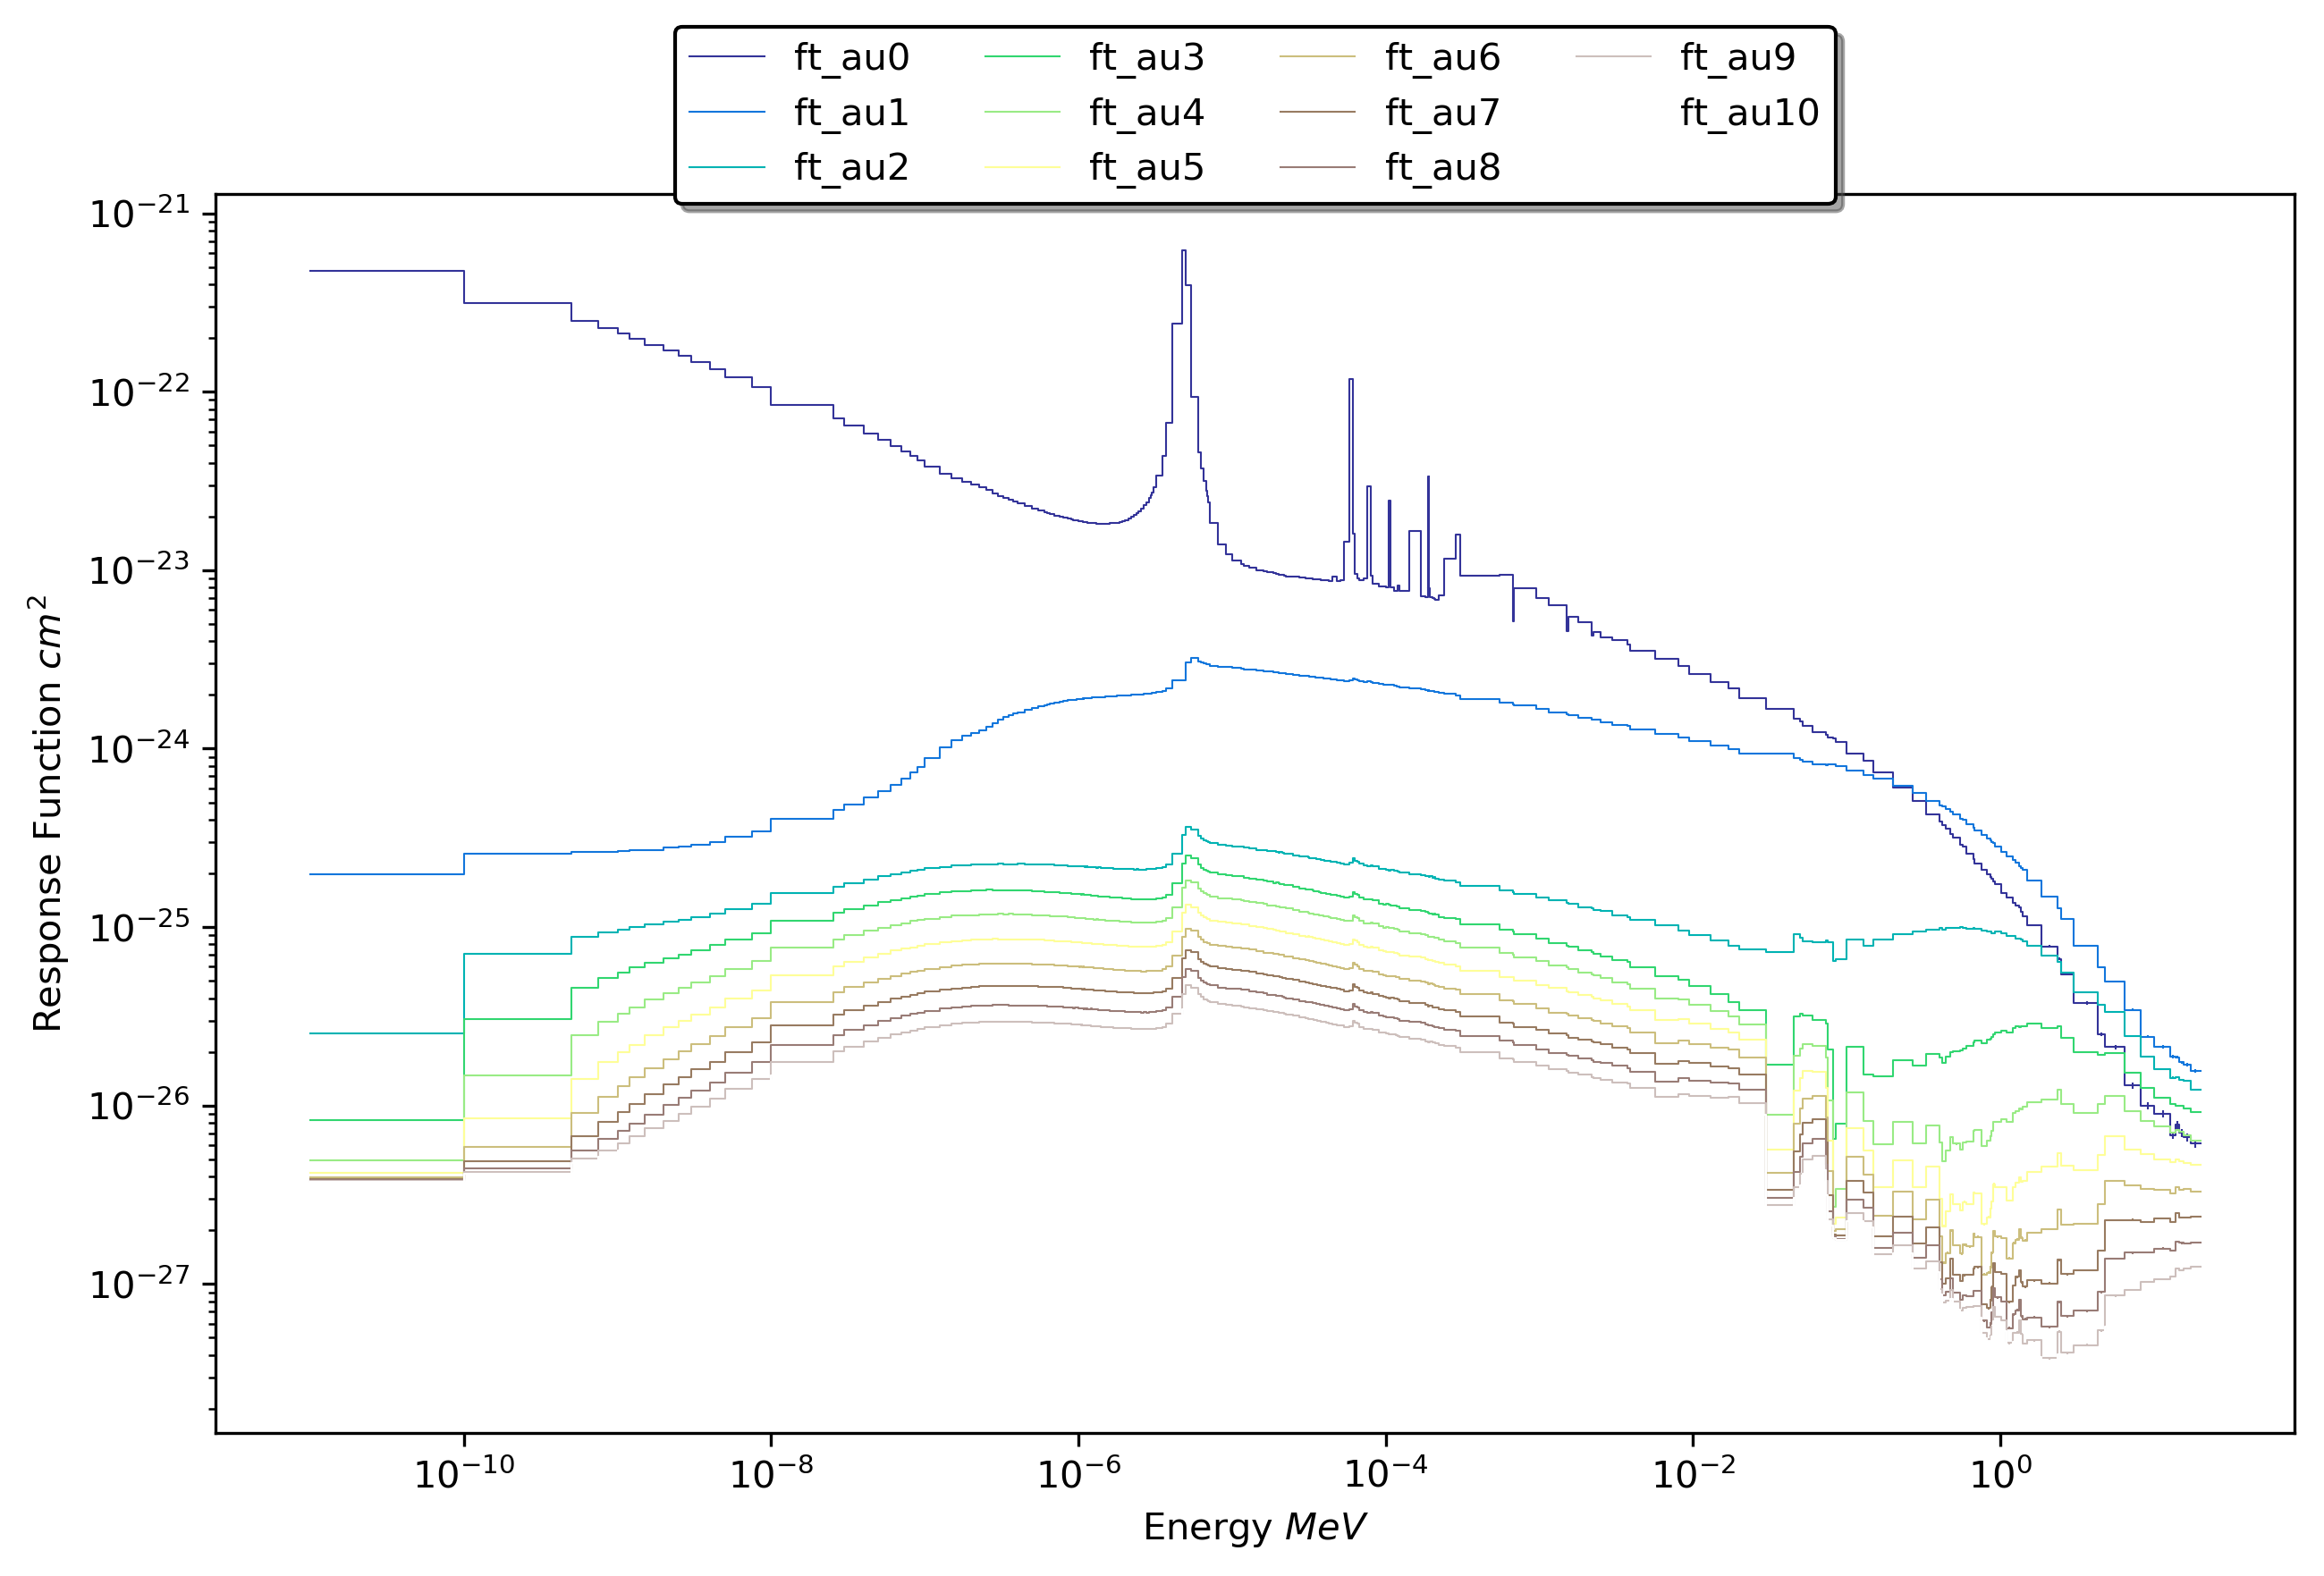
\includegraphics[width = 0.8\textwidth]{ft_au}
\caption{The MCNP-generated response functions for the gold foil tube detector.}
\end{figure}

\end{frame}

%%%%%%%%%%%%%%%%%%%%% bonner sphere response functions
\begin{frame}
\frametitle{Bonner Sphere Response Functions}

\begin{figure}
\centering
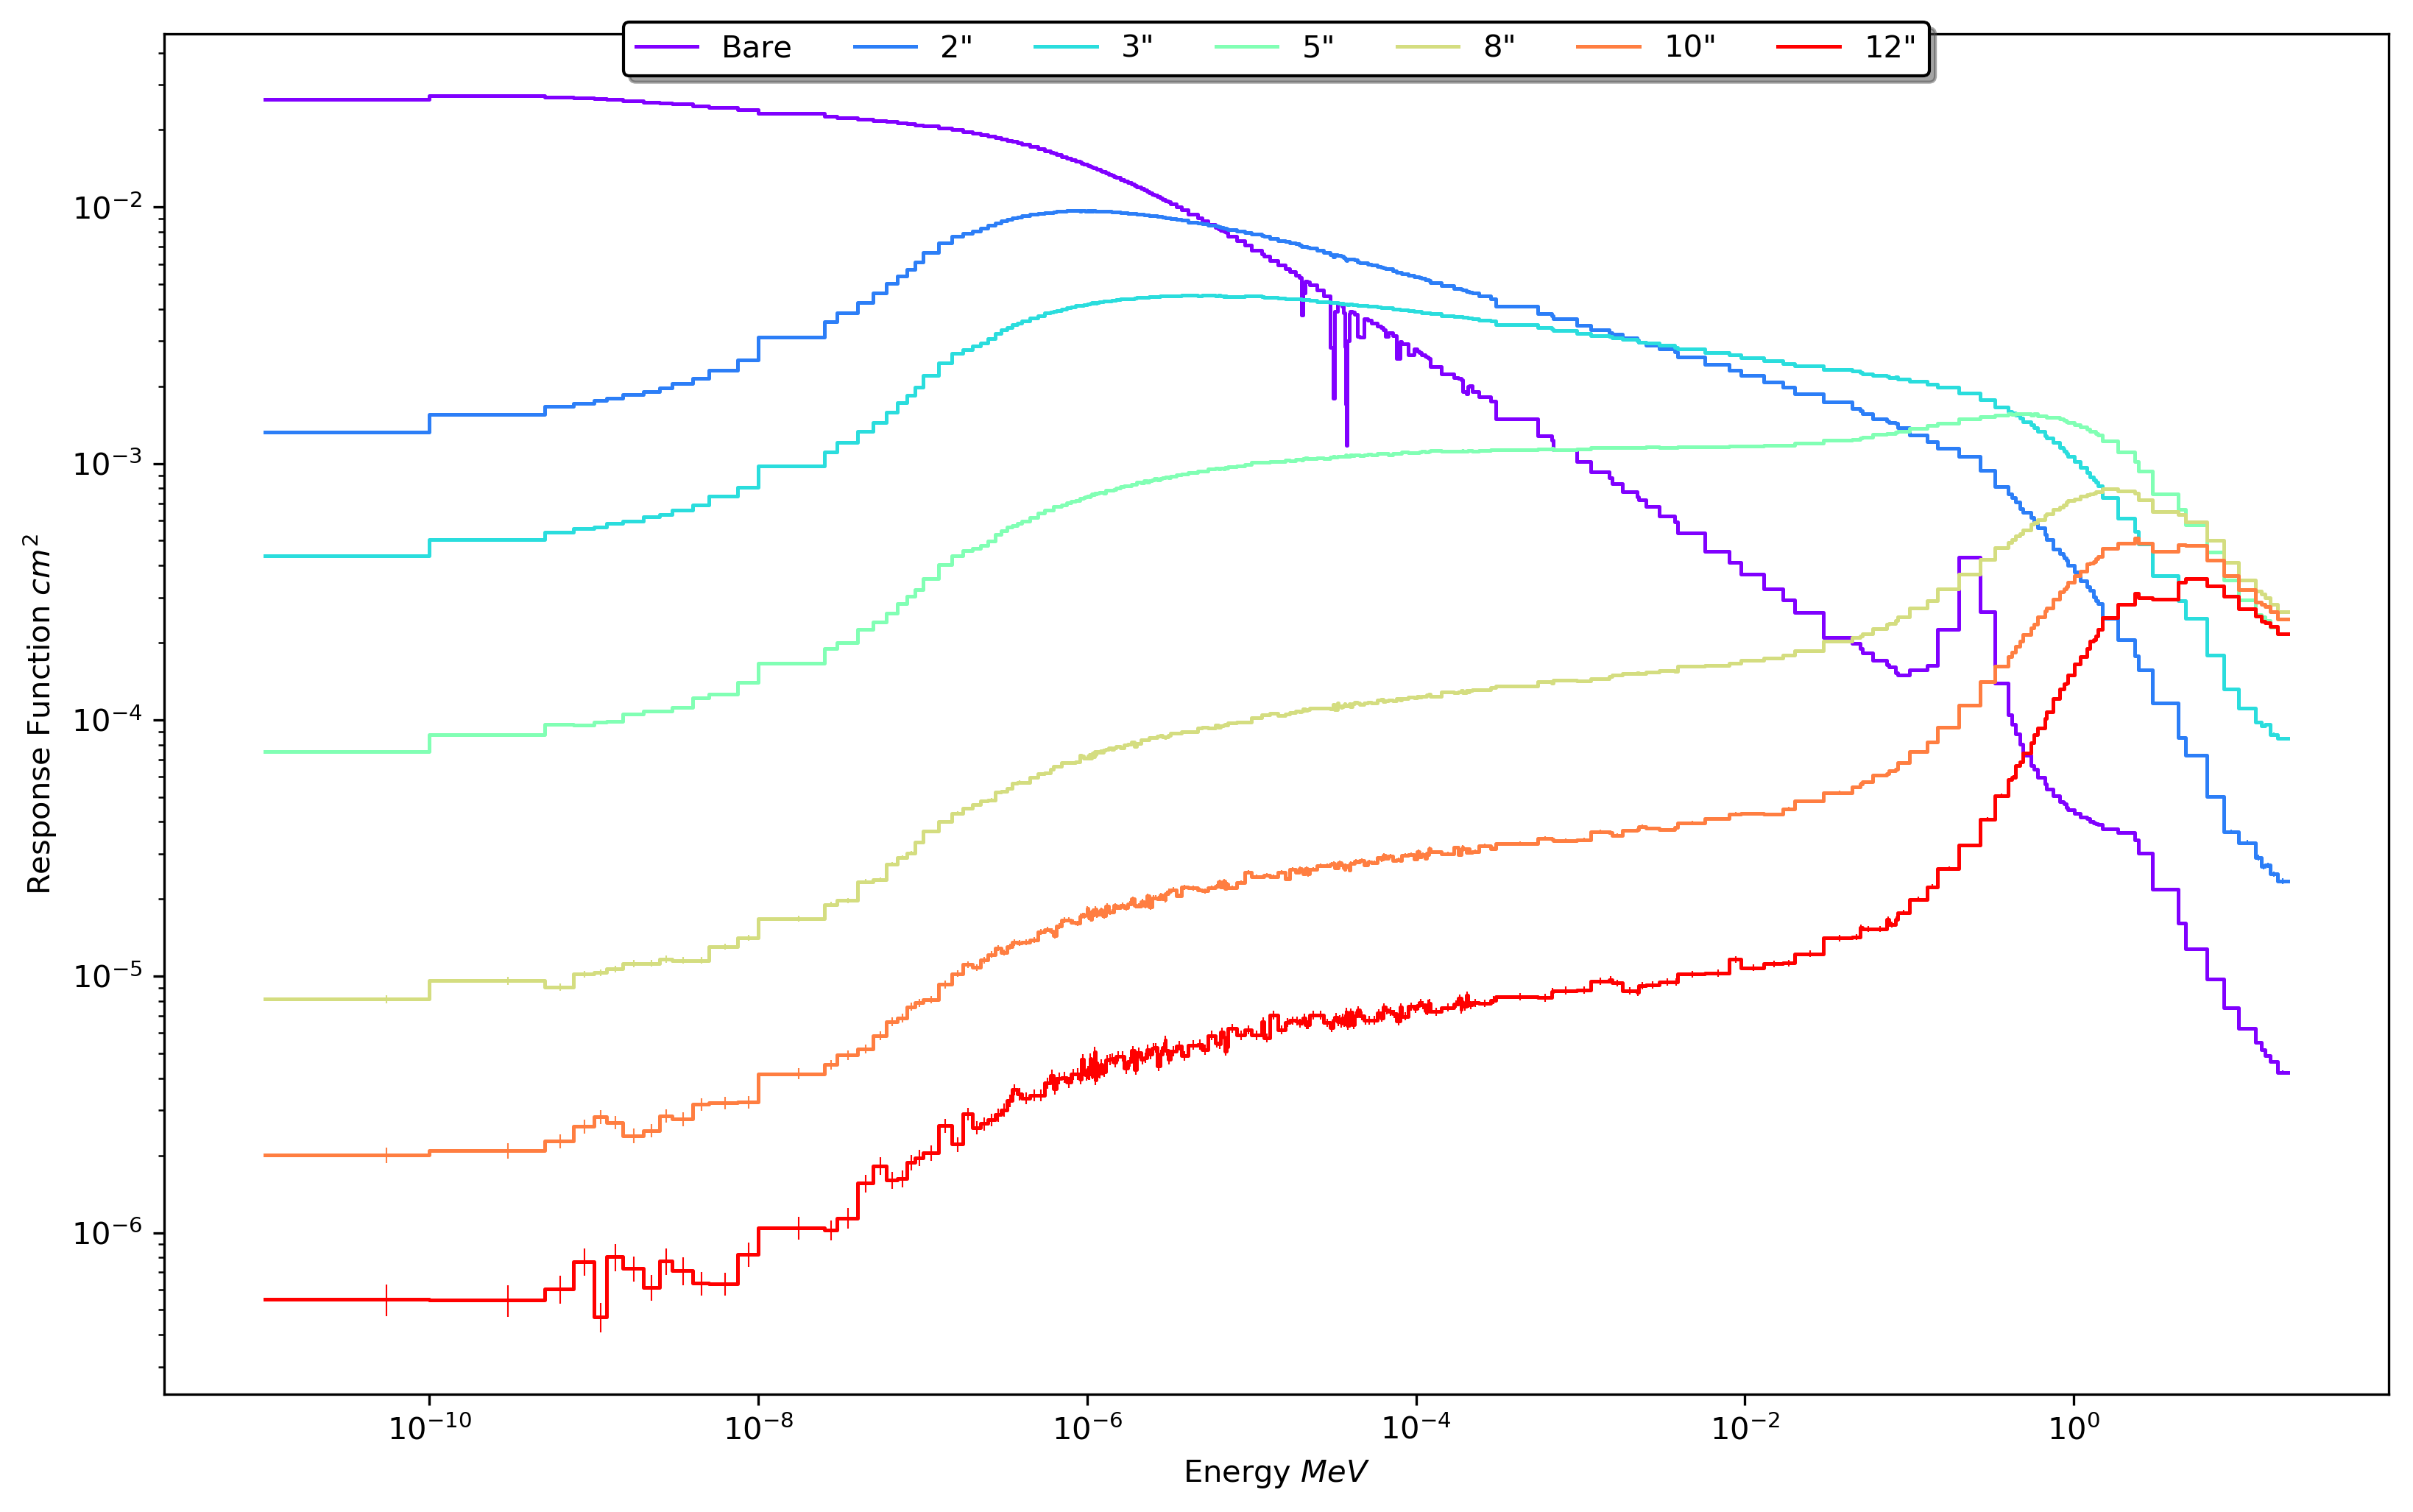
\includegraphics[width = 0.8\textwidth]{bs}
\caption{The MCNP-generated response functions for the bonner sphere spectrometer.}
\end{figure}

\end{frame}

%%%%%%%%%%%%%%%%%%%%% experimental procedures: ft
\begin{frame}
\frametitle{Experimental Procedures}

Gold foil tube
\begin{itemize}
\item Tube inserted into NEBP collimator.
\item Reactor brought to 100 kW(th).
\item Irradiated for approximately 2.5 hours.
\item Reactor powered off, foils removed from tube, bagged and labeled.
\item Foils counted with HPGe
\end{itemize}

Bonner Sphere Spectrometer
\begin{itemize}
\item Reactor powered to 1 kW(th).
\item Bare detector placed directly in front of beam 28" from aperture.
\item Shutter opened
\item Aquired counts for 300s live time (600s for 12" sphere).
\item Shutter closed
\item Repeated for different spheres (2", 3", 5", 8", 10", 12").
\end{itemize}
\end{frame}

%%%%%%%%%%%%%%%%%%%%% gold foil post processing
\begin{frame}
\frametitle{Foil Tube Postprocessing}

\begin{equation}
\label{eqn:a_sat}
A_{sat} = A_{meas} \frac{R_{meas}}{R_{sat} n_a K I_{rel}} ,
\end{equation}

$A_{meas}$ is the measured activity\\
$R_{meas}$ corrects for decay during measurement\\
$R_{sat}$ is the ratio between the radiation at measurement and the saturation activity\\
$n_a$ is the number of sample atoms\\
$K$ is the isotopic abundance\\
$I_{rel}$ is the relative gamma intensity\\

\end{frame}

%%%%%%%%%%%%%%%%%%%%% transient mathematics
\begin{frame}
\frametitle{Capturing Flux Transients}

\begin{equation}
\label{eqn:bateman_r_sat}
\frac{R_{sat}(t)}{dt} = \lambda (P_{f}(t) - R_{sat}(t))
\end{equation}

$\lambda$ is the decay constant\\
$P_f(t)$ is the power at time $t$ relative to nominal power

\vspace{0.05\textheight}

Allows for {\it transient} power data to be used when calculating saturation activities!

\end{frame}


%%%%%%%%%%%%%%%%%%%%% bss postprocessing
\begin{frame}
\frametitle{Bonner Sphere Postprocessing}

\begin{figure}
\centering
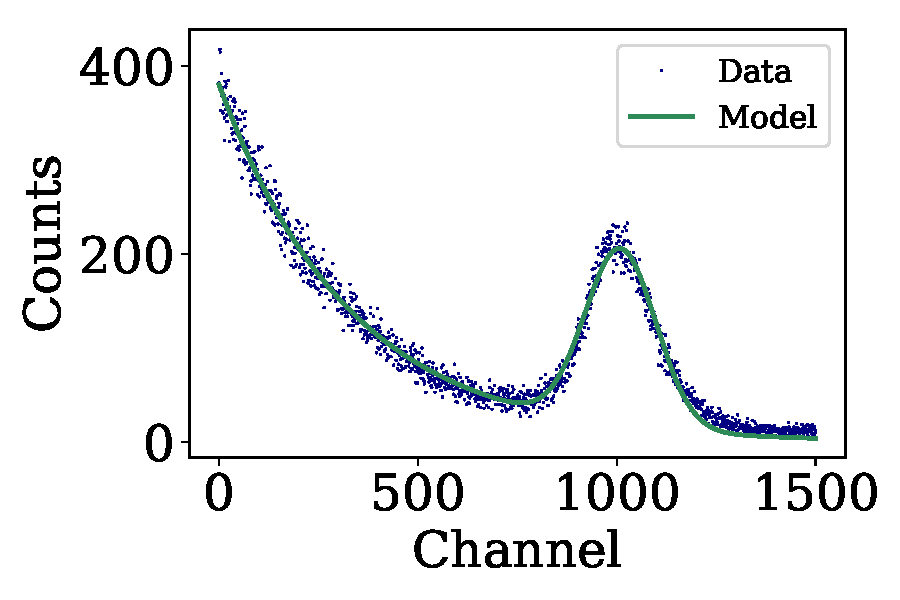
\includegraphics[width = 0.7\textwidth]{bs4_spectrum}
\caption{The aquired spectrum from the 8" sphere and model used to find the response.}
\end{figure}

\end{frame}

%%%%%%%%%%%%%%%%%%%%% response comparison: ft
\begin{frame}
\frametitle{Response Comparison: Foil Tube}

\begin{figure}
\centering
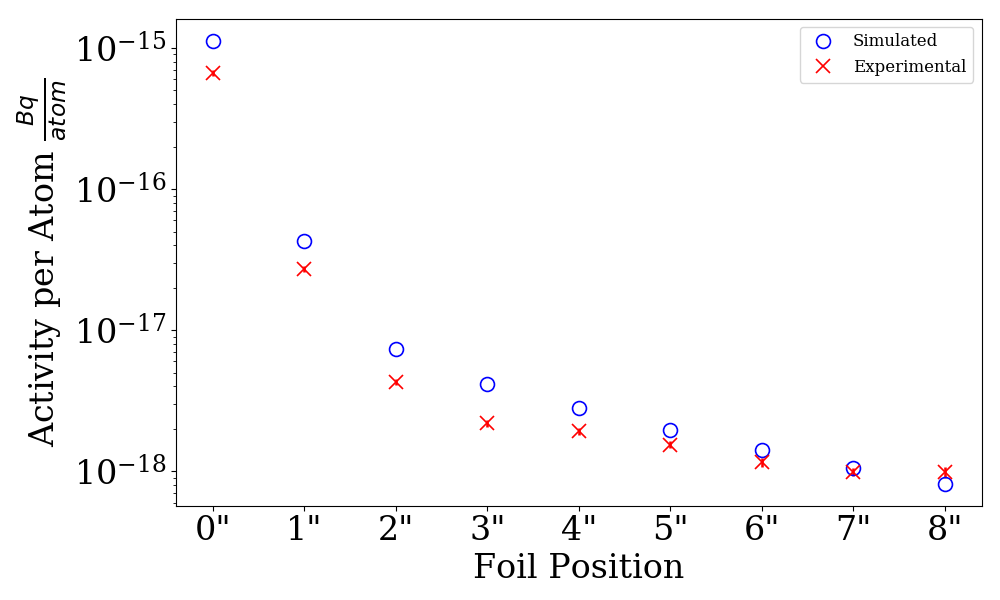
\includegraphics[width = 0.8\textwidth]{compare_activities}
\caption{A comparison of the simulated and experimentally determined activites for the gold foil tube.}
\end{figure}

\end{frame}

%%%%%%%%%%%%%%%%%%%%% response comparison: bss
\begin{frame}
\frametitle{Response Comparison: Bonner Sphere}

\begin{figure}
\centering
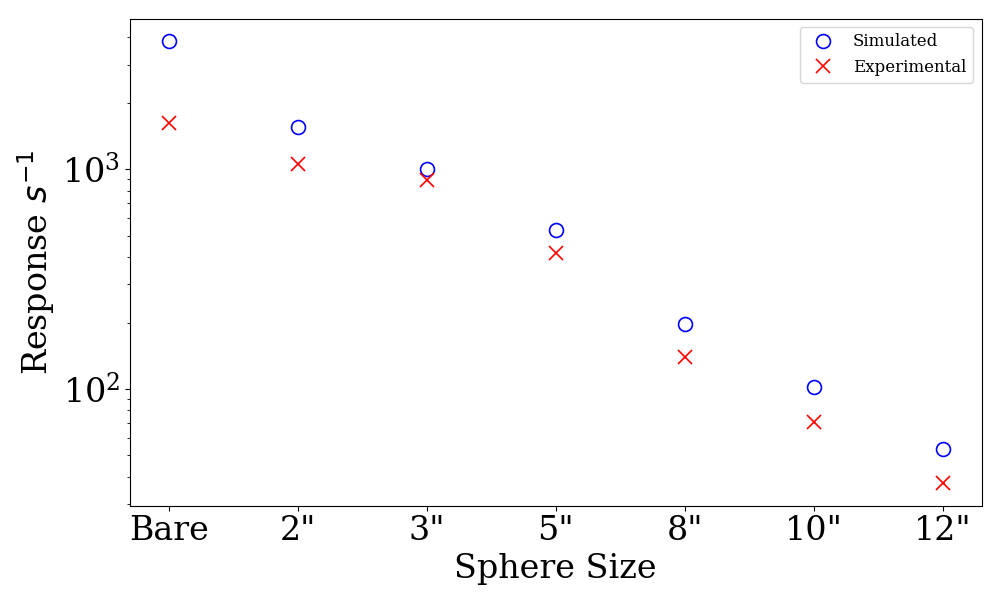
\includegraphics[width = 0.8\textwidth]{compare_countrates}
\caption{A comparison of the simulated and experimentally determined count rates for the bonner sphere spectrometer.}
\end{figure}

\end{frame}

%%%%%%%%%%%%%%%%%%%%% spectral unfolding: parameters
\begin{frame}
\frametitle{Spectral Unfolding Parameters}

Doroshenko Directed Divergence
\begin{itemize}
\item 50 iterations
\end{itemize}

Gravel
\begin{itemize}
\item 50 iterations
\end{itemize}

MAXED
\begin{itemize}
\item Omega = 9 (foil tube), 7 (BSS), 16 (combined)
\item With and without pre-scaling default spectrum magnitude
\end{itemize}

\end{frame}

%%%%%%%%%%%%%%%%%%%%% spectral unfolding: doroshenko
\begin{frame}
\frametitle{Spectral Unfolding: Doroshenko Directed Divergence}

\begin{figure}
\centering
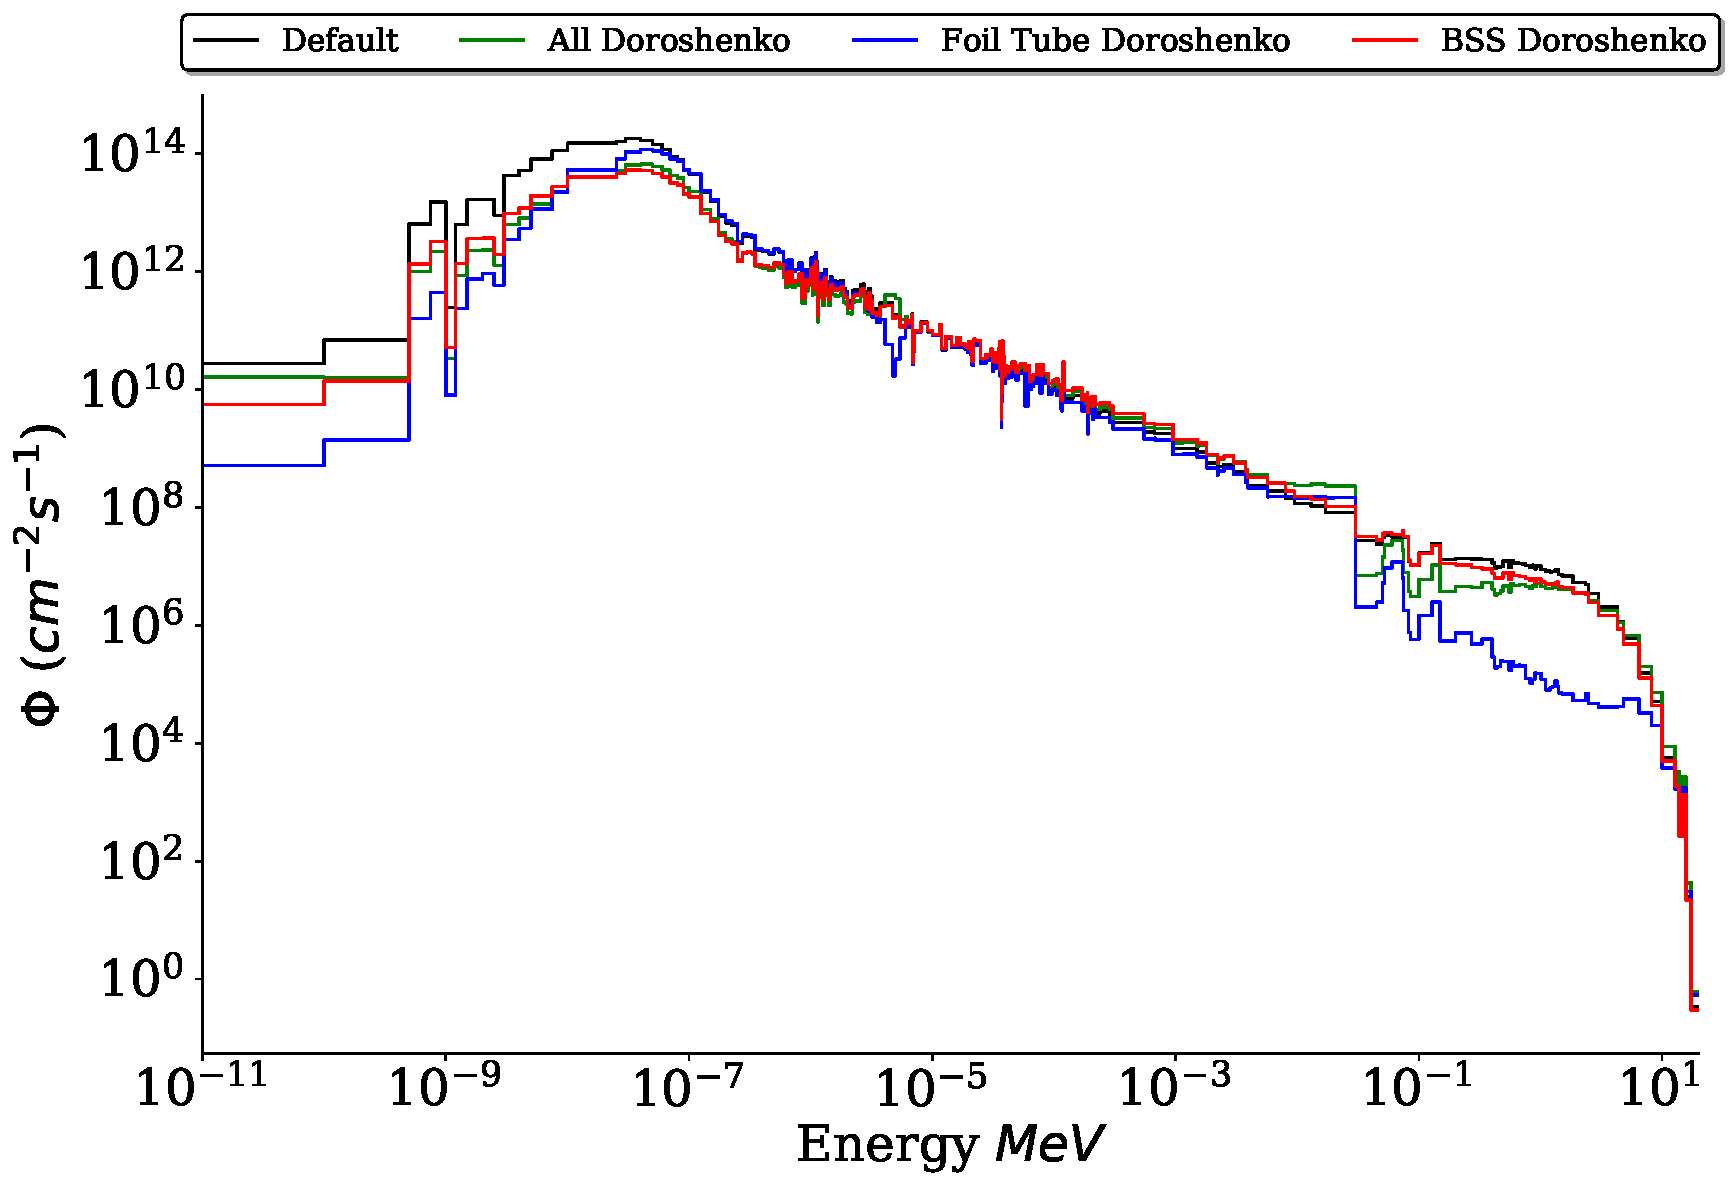
\includegraphics[width = 0.8\textwidth]{unfolded_do}
\caption{The unfolded spectra from Doroshenko Directed Divergence.}
\end{figure}

\end{frame}

%%%%%%%%%%%%%%%%%%%%% spectral unfolding: gravel
\begin{frame}
\frametitle{Spectral Unfolding: Gravel}

\begin{figure}
\centering
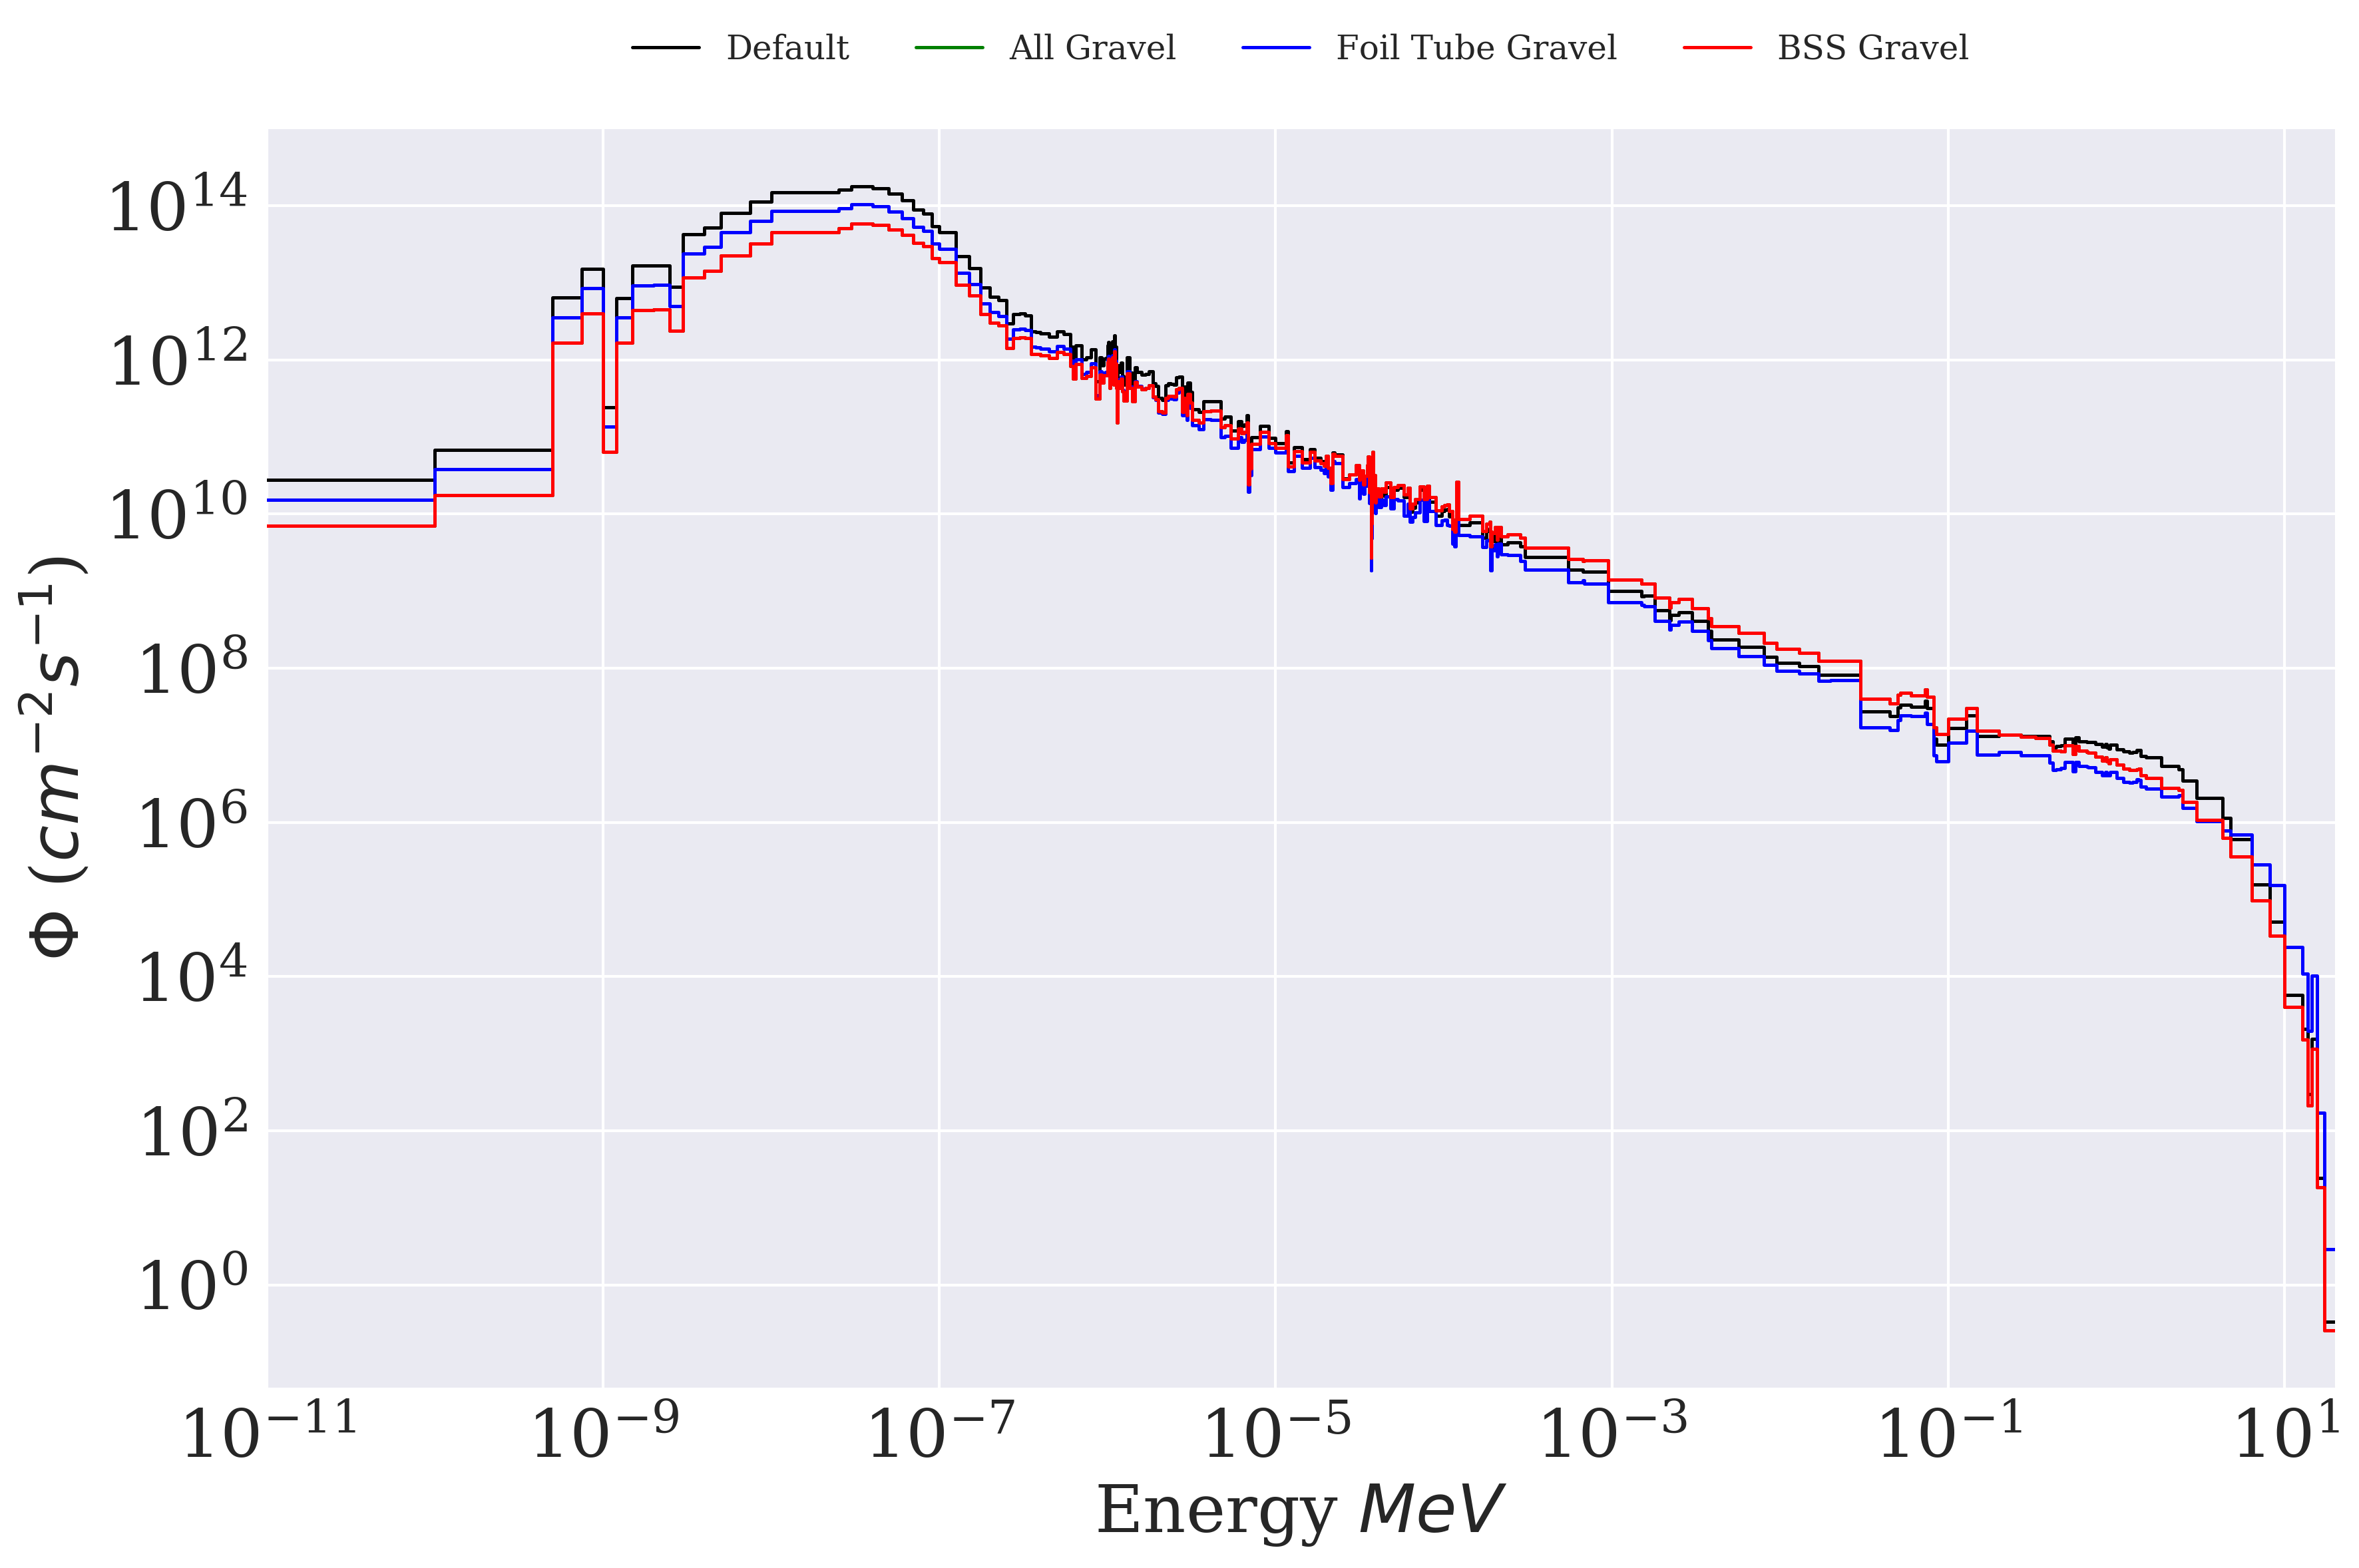
\includegraphics[width = 0.8\textwidth]{unfolded_gr}
\caption{The unfolded spectra from Gravel.}
\end{figure}

\end{frame}

%%%%%%%%%%%%%%%%%%%%% spectral unfolding: maxed
\begin{frame}
\frametitle{Spectral Unfolding MAXED}

\begin{figure}
\centering
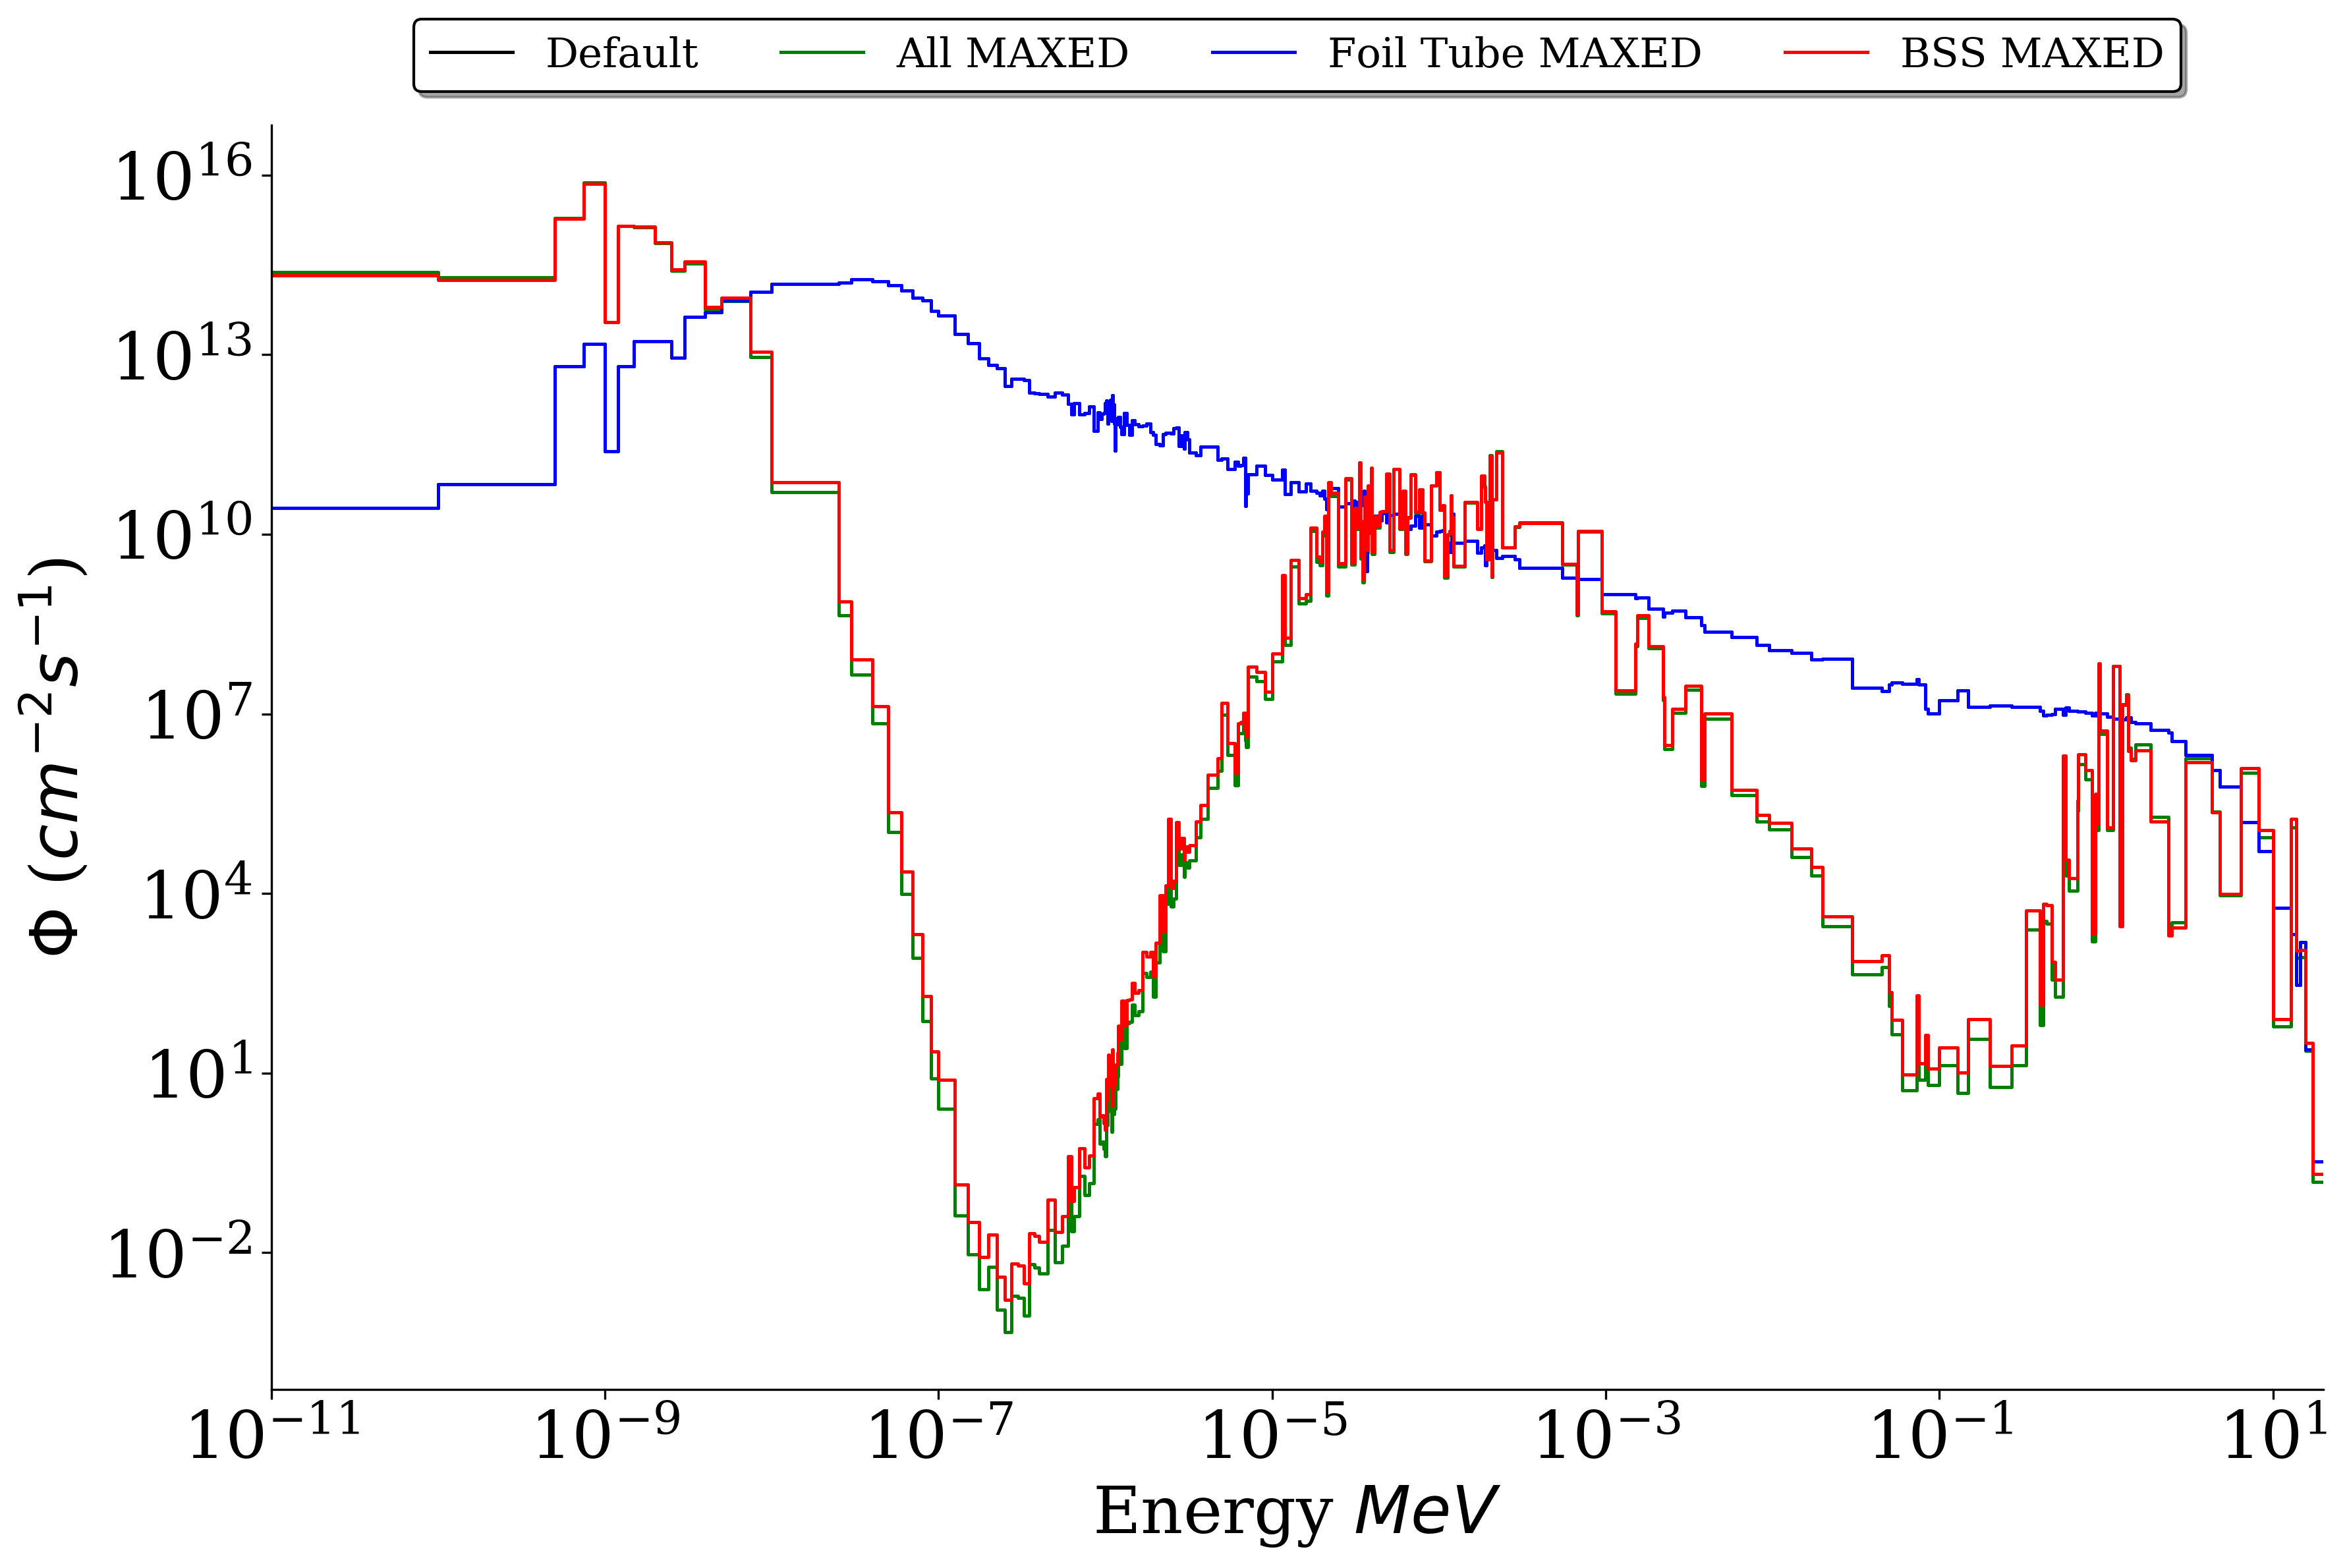
\includegraphics[width = 0.8\textwidth]{unfolded_mx}
\caption{The unfolded spectra from MAXED.}
\end{figure}

\end{frame}

\begin{frame}
\frametitle{Spectral Unfolding MAXED (Scaled)}

\begin{figure}
\centering
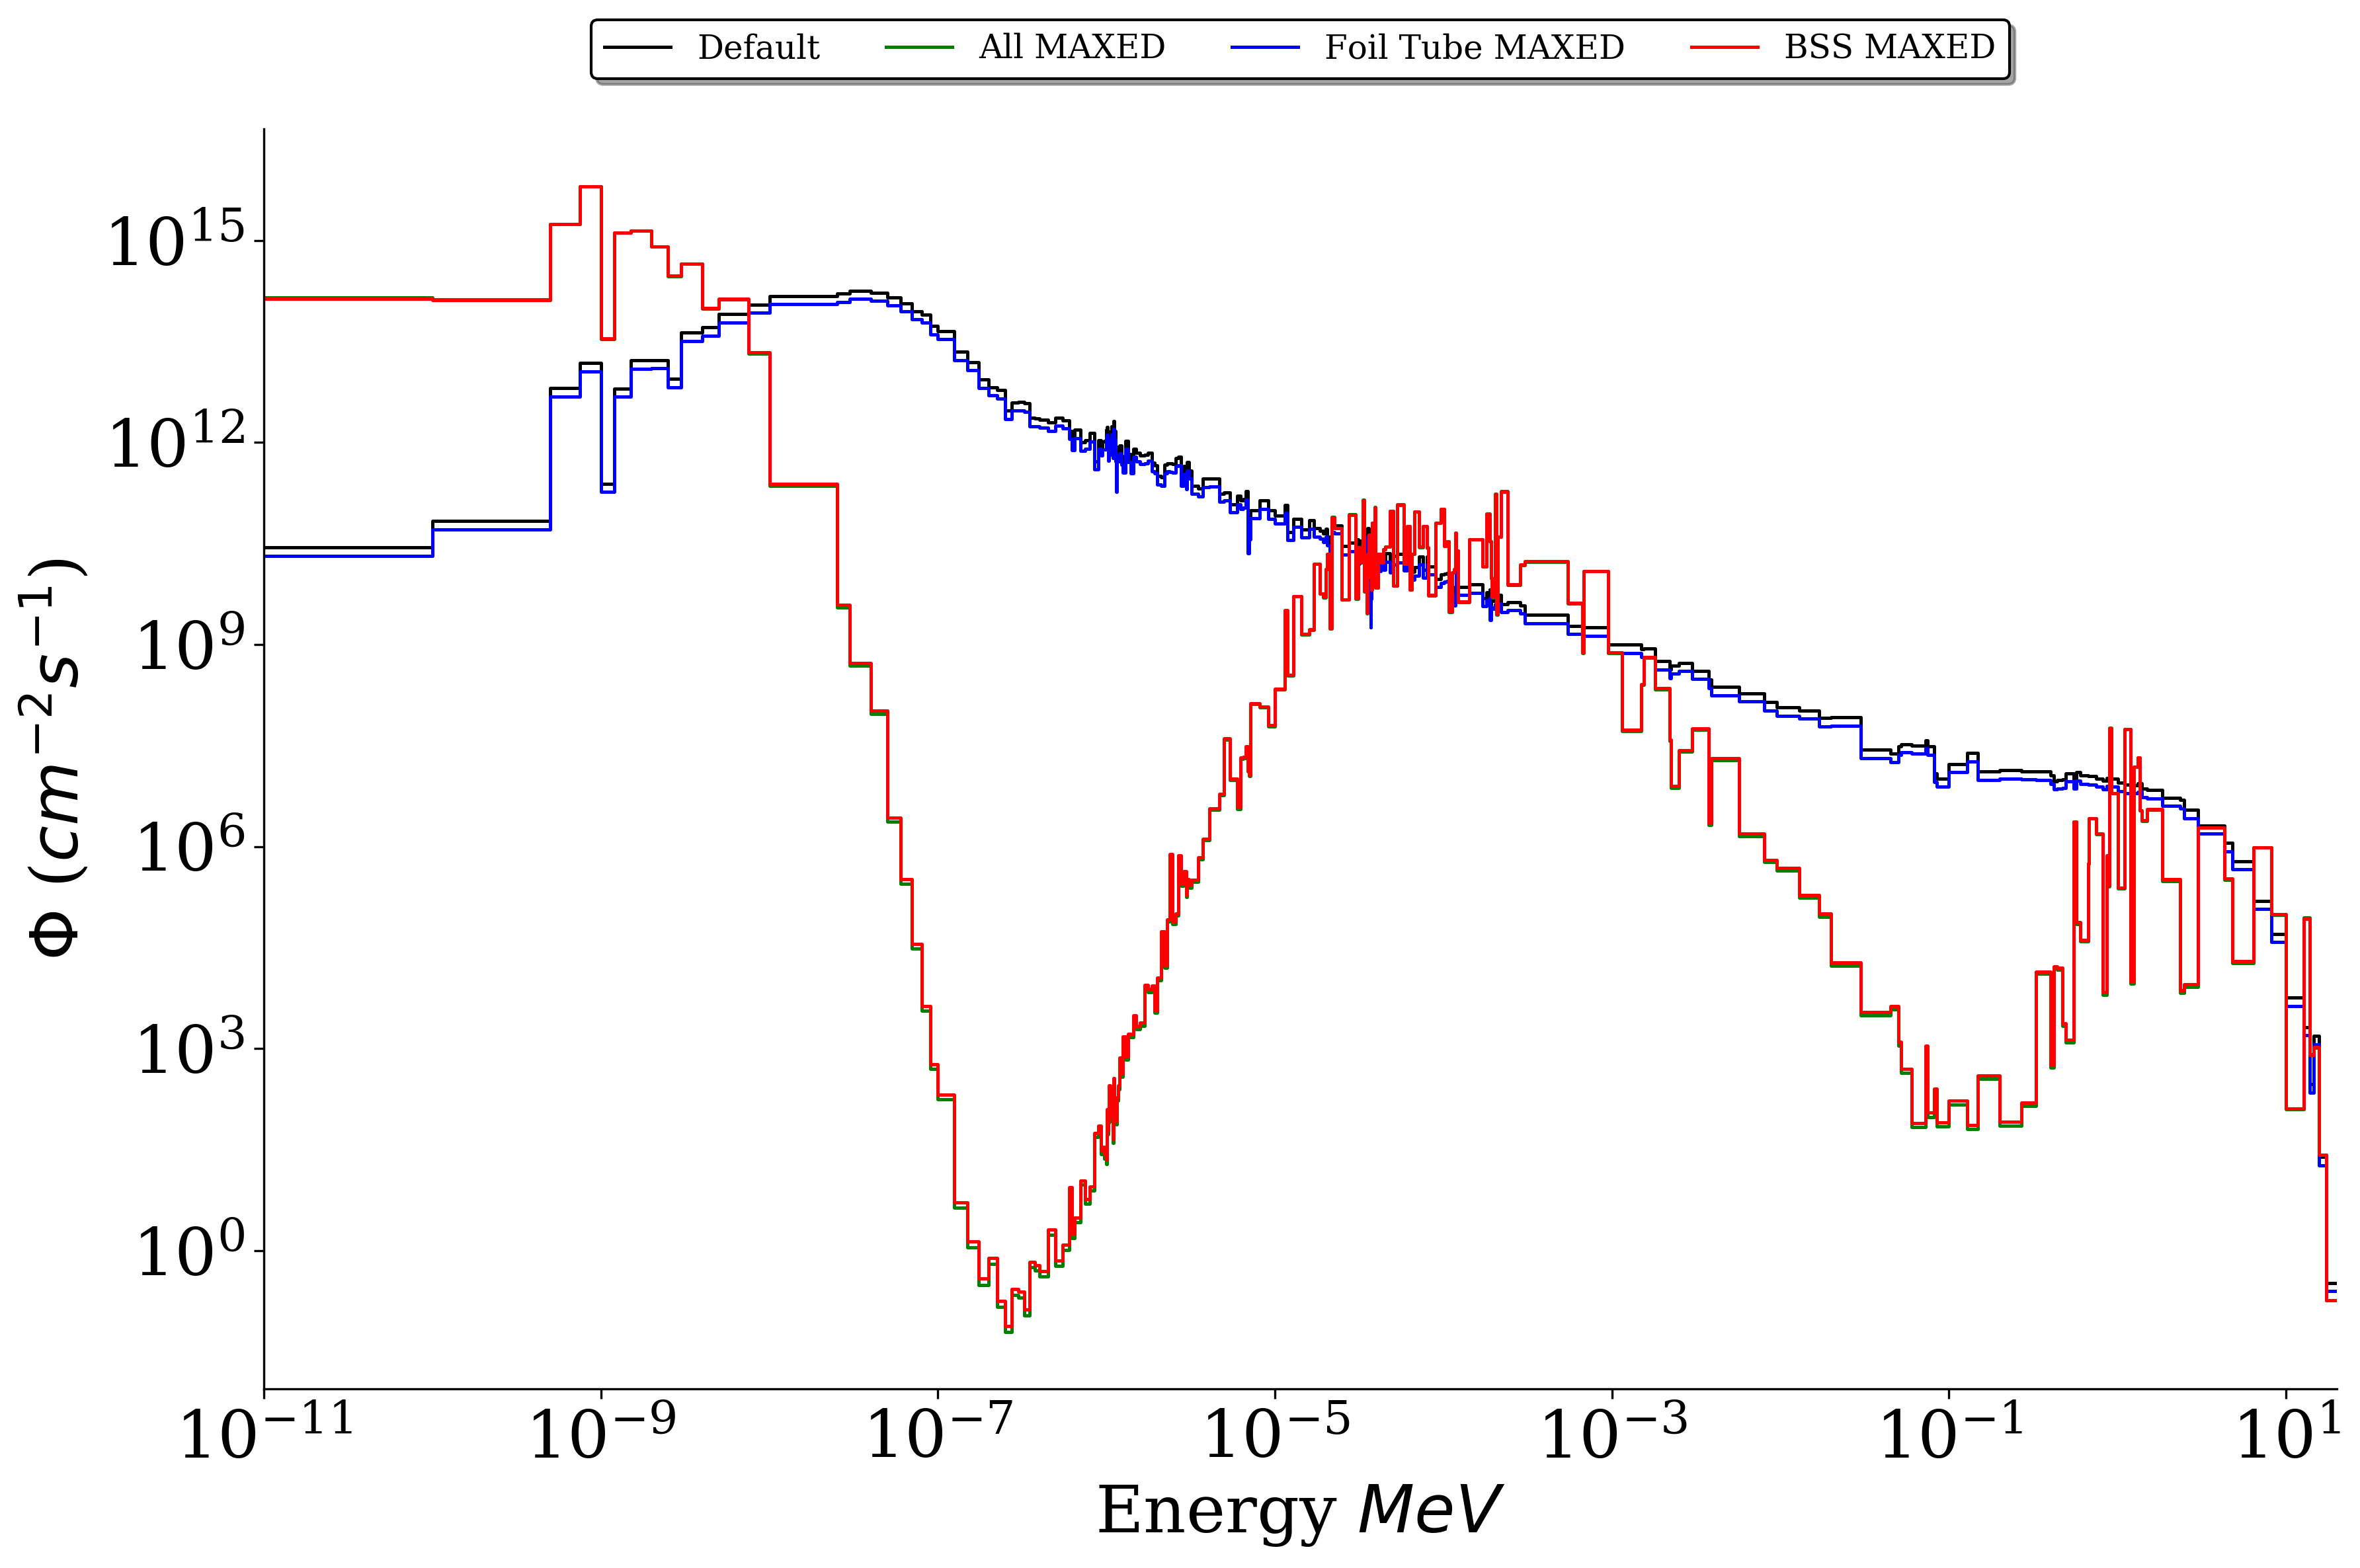
\includegraphics[width = 0.8\textwidth]{unfolded_mx_sc}
\caption{The unfolded spectra from MAXED (scaled).}
\end{figure}

\end{frame}

%%% Conclusions & Future Work (3) ---------------------------------------------------------------------------------------
\section{Conclusions and Future Work}

%%%%%%%%%%%%%%%%%%%%% buffer slide
\begin{frame}
\frametitle{Conclusions and Future Work}

Conclusions drawn from the experiment and motivation for future work

\end{frame}
%%%%%%%%%%%%%%%%%%%%% conclusions
\begin{frame}
\frametitle{Conclusions}
\begin{itemize}
\item Multi-dimensional, high resolution flux simulated
\item Active and passive detection experiments conducted
\item Final spectra unfolded with multiple methods
\item Flux was predominantly monodirectional, but not as fast as expected
\end{itemize}

\end{frame}

%%%%%%%%%%%%%%%%%%%%% future work
\begin{frame}
\frametitle{Future Work}
\begin{itemize}
\item Characterization of other beam ports
\item Continued optimization of foil tube design
\end{itemize}
\end{frame}

%%%%%%%%%%%%%%%%%%%%% references
\begin{frame}[t,allowframebreaks]\label{lastframe}
\frametitle{References}
\bibliographystyle{ans}
% make a bibliography.bib file with your references in it
{\scriptsize
\bibliography{references}}
\end{frame}


\end{document}



